% Copyright 2013 Nicolai Hähnle <nhaehnle@gmail.com>
%
% This work is licensed under the Creative Commons Attribution-ShareAlike 3.0
% Unported License, see http://creativecommons.org/licenses/by-sa/3.0/
%
% Among other things, this means that yes, you may take e.g. illustrations from
% the book and use them in your own work. However, (a) you must give proper
% attribution by naming me as its original author and (b) you must make your
% derivative work available under the same or similar license terms.
%
% See the Creative Commons website for the exact licensing terms.

\chapter{Generating Functions and the Algebra of Polyhedra}

We have seen how to enumerate the lattice points in a convex body $K$
in time that is essentially proportional to the maximum number of lattice points
in a translate of $K$.
What if we are only interested in the \emph{number} $|K \cap \Lambda|$ of such points?

Throughout this chapter, we will work with $\Lambda = \Z^d$ -- using a linear transformation,
this is without loss of generality.
Consider the box $K = [0,M]^d$.
It contains roughly $M^d$ integer points, which is exponential in the number of bits
required to encode a description of $K$.
On the other hand, computing this number is a trivial task that can be performed in
polynomial time in the encoding length of $K$.
This leads us to suspect that \emph{computing the number} of integer points could be
exponentially faster than \emph{enumerating} all those points.

In the case of a box,
computing the number of points is a polynomial problem even when the dimension $d$ is allowed to vary.
We do not expect this to be true in general
because the problem of deciding whether $|P \cap \Z^d| = 0$ for an arbitrary polytope $P$ is the integer programming problem,
which is $NP$-hard.
In fact, computing $|P \cap \Z^d|$ is easily seen to be a $\# P$-hard problem.
So we should contend ourselves with looking for an algorithm that is polynomial so long as $d$ is fixed,
and with trying to reduce the dependence on $d$ of the degree of this polynomial.

The enumeration algorithms of the last chapter could be formulated with representations of convex bodies via oracles.
This is no longer the case for computing the number of integer points.
Let $N \in \N$ and consider the convex body
\[
  K_\varepsilon(a,b) := \{ (x,y) \in \R^2 ~:~ a \leq x \leq b, xy \geq N + \varepsilon, y \leq N \}
\]
The lower envelope of $K_0(a, b)$ contains an integer point if and only if $N$ has a factor between $a$ and $b$,
see Figure~\ref{fig:factoring-body}.
Consequently, for $\varepsilon \in (0,1)$ one has $|K_0 \cap \Z^2| - |K_\varepsilon \cap \Z^2| > 0$ if and only if $N$ has a factor between $a$ and $b$.
\begin{fact}
  If there were a polynomial-time algorithm for computing the number of integer points in (somewhat general) convex bodies in $\R^2$,
  then one could factor integers in polynomial time.
\end{fact}
We do not expect factoring to be a polynomial time problem,
so we cannot hope to count integer points in arbitrary convex bodies efficiently.
Instead, our goal will be a polynomial time algorithm that counts the number of integer points in \emph{polytopes}
in fixed dimension.

\begin{figure}
  \begin{center}
    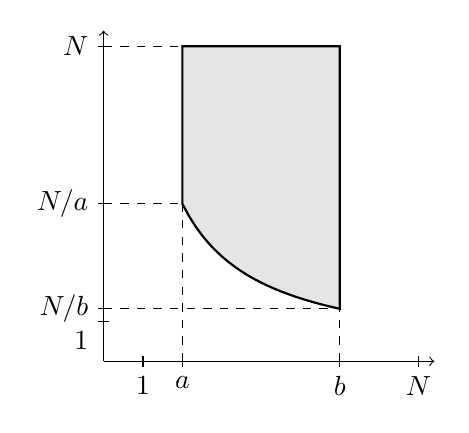
\begin{tikzpicture}
      \draw[->] (0,0) -- (4.2,0);
      \draw[->] (0,0) -- (0,4.2);

      \draw[dashed] (0,0.666) -- (3,0.666);
      \draw[dashed] (0,2) -- (1,2);
      \draw[dashed] (0,4) -- (1,4);

      \draw[dashed] (1,0) -- (1,2);
      \draw[dashed] (3,0) -- (3,0.666);

      \draw (0.5,0) +(0,2pt) -- +(0,-2pt) node[below] {$1$};
      \draw (1,0) +(0,2pt) -- +(0,-2pt) node[below] {$a$};
      \draw (3,0) +(0,2pt) -- +(0,-2pt) node[below] {$b$};
      \draw (4,0) +(0,2pt) -- +(0,-2pt) node[below] {$N$};
      \draw (0,0.5) +(2pt,0) -- +(-2pt,0) node[below left] {$1$};
      \draw (0,2) +(2pt,0) -- +(-2pt,0) node[left] {$N/a$};
      \draw (0,0.666) +(2pt,0) -- +(-2pt,0) node[left] {$N/b$};
      \draw (0,4) +(2pt,0) -- +(-2pt,0) node[left] {$N$};

      \draw[thick,fill=black!10] plot[domain=1:3] (\x, {2 / \x}) -- (3,4) -- (1,4) -- cycle;
    \end{tikzpicture}
  \end{center}
  \caption{The body $K_0(a,b)$ encodes information about the factors of $N$.}
  \label{fig:factoring-body}
\end{figure}



\section{A simple example of generating functions}
\label{sec:simple-example-generating-functions}

Suppose we want to count the number of integer points in an interval $I := [a,b] \subset \R$
in a way that might be extendable to higher dimension.
One way of doing this is to symbolically determine the \emph{generating function}
\[
  f(I;x) = \sum_{p \in I \cap \Z} x^p
\]
and evaluate it at the point $f(I;1) = |I \cap \Z|$.
Unfortunately, $f(I;x)$ is the sum of $|I \cap \Z|$ monomials,
and so the memory space required for writing this sum down is exponential in the encoding length of $I$.
A better approach is needed. The geometric series
\[
  \sum_{p = 0}^\infty x^p
\]
is the generating function of the unbounded interval $[0,\infty)$
and satisfies
\[
  \sum_{p = 0}^\infty x^p = \frac{1}{1 - x}
\]
where the series converges absolutely.
The following picture suggest a way to leverage the geometric series for our problem:
\begin{center}
  \begin{tikzpicture}
    \draw (-0.2,0) -- (8.2,0);
    \foreach \x in {0,0.5,...,8.01}
      \draw (\x,0) +(0,2pt) -- +(0,-2pt);

    \draw[very thick] (2,0) node[below] {$a$} -- node[above] {$I$} (5,0) node[below] {$b$};

    \draw (2,-1) +(0,2pt) -- +(0,-2pt) +(0,0) -- (8.2,-1);
    \draw (5.5,-1.5) +(0,2pt) -- +(0,-2pt) +(0,0) -- (8.2,-1.5);

    \draw (1,-1) node {$=$};
    \draw (1,-1.5) node {$-$};
  \end{tikzpicture}
\end{center}
The graphical ``formula'' carries over to formal Laurent series (assuming $a, b \in \Z$ for simplicity):
\[
  \sum_{p = a}^b x^p = \sum_{p = a}^\infty x^p - \sum_{p = b+1}^\infty x^p
\]
There is an open set $U \subset \C$ on which all series converge absolutely,
and so
\[
  \sum_{p = a}^b x^p = \frac{x^a}{1 - x} - \frac{x^{b + 1}}{1 - x}
\]
holds on $U$.
Since the functions involved in this equation are rational and therefore complex differentiable,
it follows that the equality must hold on all of $\C$ (except for $x = 1$, where the functions are not defined).
That is, we can write
\[
  f(I;x) = \frac{x^a}{1 - x} - \frac{x^{b + 1}}{1 - x}
\]
if we understand the equality to be up to negligible differences in the domains of the two sides of the equation.
Observe that the encoding length of the right hand side is dominated by the encodings of $a$ and $b$,
and is therefore linear in the encoding length of $I$.

The downside of this representation of $f(I;x)$ is that it is undefined at $x = 1$,
which is exactly the point where we would like to evaluate it.
However, $x = 1$ is a removable singularity.
Using the rule of de~l'Hôpital, we can compute
\[
  \lim_{x \to 1} \frac{x^a}{1 - x} - \frac{x^{b + 1}}{1 - x} = \lim_{x \to 1} \frac{x^a - x^{b+1}}{1 - x} = \lim_{x \to 1} \frac{a x^{a-1} - (b+1) x^b}{-1} = b - a + 1,
\]
which is the correct answer, as the derivation above has already shown.

Note that the graphical formula we used to derive the rational generating function for $I$ is by no means unique.
The following picture shows an alternative formula:
\begin{center}
  \begin{tikzpicture}
    \draw (-0.2,0) -- (8.2,0);
    \foreach \x in {0,0.5,...,8.01}
      \draw (\x,0) +(0,2pt) -- +(0,-2pt);

    \draw[very thick] (2,0) node[below] {$a$} -- node[above] {$I$} (5,0) node[below] {$b$};

    \draw (2,-1) +(0,2pt) -- +(0,-2pt) +(0,0) -- (8.2,-1);
    \draw (-0.2,-1.5) -- (5,-1.5)  +(0,2pt) -- +(0,-2pt);
    \draw (-0.2,-2) -- (8.2,-2);

    \draw (-1,-1) node {$=$};
    \draw (-1,-1.5) node {$+$};
    \draw (-1,-2) node {$-$};
  \end{tikzpicture}
\end{center}
Again, this carries over to formal Laurent series:
\[
  \sum_{p = a}^b x^p = \sum_{p = a}^\infty x^p + \sum_{p = -\infty}^b x^p - \sum_{p = -\infty}^\infty x^p
\]
There are two problems:
\begin{itemize}
  \item The first two series on the right hand side are geometric series for which a rational function expression is known.
    However, their regions of absolute convergence are disjoint.

  \item The last series does not converge anywhere, and it is unclear what rational function expression could be used in its place.
\end{itemize}
Over the course of this chapter,
we will see that the first problem turns out not to be a problem after all,
and that the last, non-converging series, magically disappears.
One finds that
\[
  f(I;x) = \frac{x^a}{1-x} + \frac{x^b}{1-x^{-1}}
\]
where, again, the equality should be understood modulo negligible differences in the functions' domains.
For now, the reader may want to convince themselves that the equation above does indeed hold in this particular case,
for example by manual comparison to the rational function obtained previously.

The remainder of this chapter generalizes the approach we have just laid out to higher dimension,
exploring some rather fascinating algebraic structures on the way.



\section{Cones and triangulations}

\begin{definition}
  \begin{enumerate}[(a)]
    \item A non-empty convex set $K \subseteq \R^d$ is a \emph{cone}
      if $p \in K$ and $\lambda \geq 0$ imply $\lambda p \in K$.

    \item A \emph{conic combination} of vectors $u_1, \ldots, u_n \in \R^d$ is
      a linear combination with non-negative coefficients.

    \item Given $U \subset \R^d$, the set $\cone(U)$ is the set of conic combinations of vectors in $U$.

    \item A cone $K$ is \emph{polyhedral} if $K$ is a polyhedron.
  \end{enumerate}
\end{definition}

Note that cones are closed under taking conic combinations,
and $\cone{U}$ is the smallest cone containing $U$.

\begin{definition}
  Let $P$ be a non-empty polyhedron.
  The \emph{lineality space} of $P$ is
  \[
    L(P) := \{ v \in \R^d ~:~ \forall x\in P \,\forall \lambda \in \R:~ x + \lambda v \in P  \}
  \]
  If $L(P) = 0$, $P$ is called \emph{pointed}.
\end{definition}

It is not difficult to check that $L(P)$ is a linear subspace of $\R^d$.
Intuitively, $L(P)$ contains the directions of lines contained in $P$.
Polyhedra containing lines are somewhat unusual in the sense
that if one thinks of polyhedra, one usually thinks of polyhedra that have vertices,
and such polyhedra \emph{do not} contain lines.
That is, their lineality space is $0$.
However, polyhedra with lines are essential for the development of compact rational generating functions.

The following facts tie cones, polarity, and lineality spaces together.
Their proofs are left as an exercise.

\begin{lemma}
  \label{lemma:cone-polars}
  Let $K \subseteq \R^d$ be a closed cone.
  \begin{enumerate}[(a)]
    \item $K^\star = \{ y \in \R^d ~:~ y^Tx \leq 0 \,\forall\, x\in K \}$.
    \item $K^\star$ is a cone and $(K^\star)^\star = K$.
    \item $d = \dim L(K) + \dim K^\star$.
  \end{enumerate}
\end{lemma}

\begin{definition}
  A cone $K$ is \emph{simplicial} if $K = \cone\{ u_1, \ldots, u_k \}$ for linearly independent vectors $u_j \in \R^d$.
\end{definition}

\begin{definition}
  Let $K \subset \R^d$ be a full-dimensional simplicial cone,
  $K = \cone\{ u_1, \ldots, u_d \}$
  with $u_j \in \Z^d$ primitive integer vectors.
  Then the \emph{determinant} of $K$ is
  \[
    \det(K) := |\det(u_1,\ldots,u_d)|
  \]
  A \emph{unimodular} cone is a full-dimensional simplicial cone with determinant $1$.
\end{definition}

Again, the proofs of the following facts about simplicial and unimodular cones are left as an exercise.

\begin{lemma}
  \label{lemma:simplicial-cone-polars}
  Let $K = \cone\{u_1,\ldots,u_d\} \subset \R^d$ be a full-dimensional simplicial cone.
  \begin{enumerate}[(a)]
    \item Let $A = (u_1, \ldots, u_d)$. Then $K = \{ p \in \R^d ~:~ -A^{-1} p \leq 0 \}$.
    \item $K^\star$ is simplicial.
    \item $K$ is unimodular if and only if $K^\star$ is unimodular.
  \end{enumerate}
\end{lemma}

\begin{figure}
  \begin{center}
    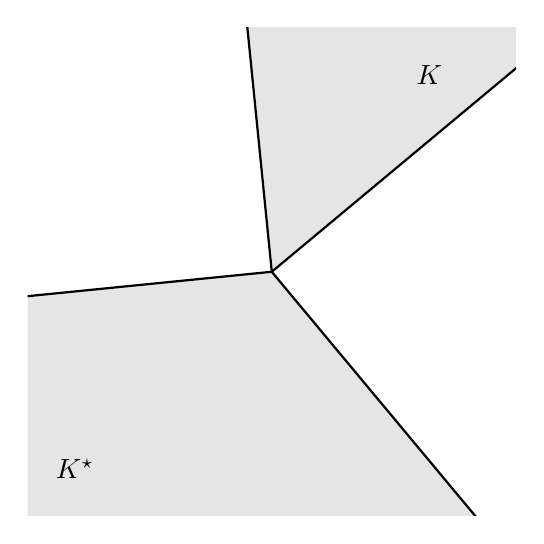
\begin{tikzpicture}
      \clip (-3.1,-3.1) rectangle (3.1,3.1);

      \draw[thick,fill=black!10] (-0.5,5) -- (0,0) -- (6,5);
      \draw[thick,fill=black!10] (-10,-1) -- (0,0) -- (10,-12);
      \draw (2,2.5) node {$K$};
      \draw (-2.5,-2.5) node {$K^\star$};
    \end{tikzpicture}
  \end{center}
  \caption{A simplicial cone and its polar.}
\end{figure}


Working with simplicial cones is desirable due to their simple combinatorial structure.
For this reason, we want to \emph{triangulate} more complicated polyhedral cones into simplicial cones.
We start by defining the notion of triangulation for polytopes,
see Figure~\ref{fig:triangulation-example}.

\begin{definition}
  Let $P \subset \R^d$ be a polytope.
  A set of simplices $\Delta_1, \ldots, \Delta_n$ is a \emph{triangulation} of $P$ if
  \begin{enumerate}
    \item $P = \bigcup_j \Delta_j$ and
    \item for every $i \neq j$, $\Delta_i \cap \Delta_j$ is a face of both $\Delta_i$ and $\Delta_j$ (possibly the empty face).
  \end{enumerate}
\end{definition}

\begin{figure}
  \begin{center}
    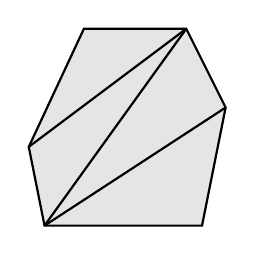
\begin{tikzpicture}
      \coordinate (n1) at (0,0);
      \coordinate (n2) at (2,0);
      \coordinate (n3) at (2.3,1.5);
      \coordinate (n4) at (1.8,2.5);
      \coordinate (n5) at (0.5,2.5);
      \coordinate (n6) at (-0.2,1);

      \draw[thick,fill=black!10] (n1) -- (n2) -- (n3) -- (n4) -- (n5) -- (n6) -- cycle;
      \draw[thick] (n1) -- (n3);
      \draw[thick] (n1) -- (n4);
      \draw[thick] (n4) -- (n6);
    \end{tikzpicture} \qquad
    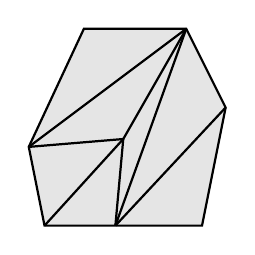
\begin{tikzpicture}
      \coordinate (n1) at (0,0);
      \coordinate (n2) at (2,0);
      \coordinate (n3) at (2.3,1.5);
      \coordinate (n4) at (1.8,2.5);
      \coordinate (n5) at (0.5,2.5);
      \coordinate (n6) at (-0.2,1);
      \coordinate (t0) at (0.9,0);
      \coordinate (t1) at (1,1.1);

      \draw[thick,fill=black!10] (n1) -- (n2) -- (n3) -- (n4) -- (n5) -- (n6) -- cycle;
      \draw[thick] (n1) -- (t1);
      \draw[thick] (n6) -- (t1);
      \draw[thick] (n4) -- (t1);
      \draw[thick] (t0) -- (n3);
      \draw[thick] (n4) -- (n6);
      \draw[thick] (t0) -- (t1);
      \draw[thick] (t0) -- (n4);
    \end{tikzpicture} \qquad
    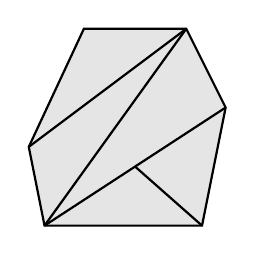
\begin{tikzpicture}
      \coordinate (n1) at (0,0);
      \coordinate (n2) at (2,0);
      \coordinate (n3) at (2.3,1.5);
      \coordinate (n4) at (1.8,2.5);
      \coordinate (n5) at (0.5,2.5);
      \coordinate (n6) at (-0.2,1);
      \coordinate (t0) at (1.15,0.75);

      \draw[thick,fill=black!10] (n1) -- (n2) -- (n3) -- (n4) -- (n5) -- (n6) -- cycle;
      \draw[thick] (n1) -- (n3);
      \draw[thick] (n1) -- (n4);
      \draw[thick] (n4) -- (n6);
      \draw[thick] (n2) -- (t0);
    \end{tikzpicture}
  \end{center}
  \caption{The first two pictures show triangulations. The last picture does not satisfy the second condition of the definition.}
  \label{fig:triangulation-example}
\end{figure}

\begin{theorem}
  \label{thm:polytope-triangulation}
  Let $P = \conv\{ v_1, \ldots, v_n \} \subset \R^d$ be a full-dimensional polytope.
  There is a triangulation $\Delta_1, \ldots, \Delta_m$ of $P$
  such that each simplex $\Delta_j$ is spanned by some subset of $d+1$ vectors from the set $\{ v_i \}_i$.

  If $P$ is rational, such a triangulation can be computed in polynomial time if $d$ is fixed.
\end{theorem}
\begin{figure}
  \begin{center}
    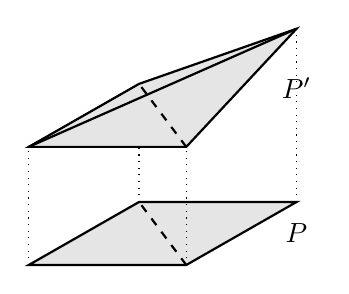
\begin{tikzpicture}
      \draw[thick,fill=black!10] (0,0) -- (2,0) -- (3.4,0.8) -- (1.4,0.8) -- cycle;

      \draw[dotted] (0,0) -- (0,1.5);
      \draw[dotted] (2,0) -- (2,1.5);
      \draw[dotted] (3.4,0.8) -- (3.4,3.0);
      \draw[dotted] (1.4,0.8) -- (1.4,2.3);

      \draw[thick,fill=black!10] (0,1.5) -- (2,1.5) -- (3.4,3.0) -- (1.4,2.3) -- cycle;
      \draw[thick,dashed] (2,1.5) -- (1.4,2.3);
      \draw[thick] (0,1.5) -- (3.4,3.0);

      \draw[thick,dashed] (2,0) -- (1.4,0.8);

      \draw (3.4,0.4) node {$P$};
      \draw (3.4,2.25) node {$P'$};
    \end{tikzpicture}
  \end{center}
  \caption{Triangulate a polytope $P \subset \R^2$ by the projection of the lower envelope of a lifting.}
  \label{fig:triangulation-proof}
\end{figure}
\begin{proof}
  The idea is to lift the vertices of $P$ into $\R^{d+1}$ in such a way
  that essentially every facet of their convex hull $P'$ is a simplex.
  The projection of the lower envelope of $P'$ will then be a triangulation of $P$,
  see Figure~\ref{fig:triangulation-proof}.

  Let us choose $t_1, \ldots, t_n \in \R$ in a manner that is to be described later
  and let $v_i' := (v_i, t_i) \in \R^{d + 1}$.
  Their convex hull
  \[
    P' := \conv\{v_1',\ldots,v_n'\}
  \]
  is a polytope with $\pi(P') = P$,
  where $\pi:\R^{d+1} \to \R^d$ is the projection onto the first $d$ coordinates.

  For every $x \in P$, let
  \[
    \ell(x) := \min\{ t ~:~ (x,t) \in P' \}.
  \]
  The point $(x, \ell(x))$ lies in a facet of $P'$
  whose defining inequality $a^Tx + \alpha t \geq \beta$ satisfies $\alpha > 0$.\footnote{This follows
  from the minimality of $\ell(x)$.}
  Let $F_1,\ldots,F_m$ be the set of facets of $P'$ whose defining inequality satisfies $\alpha > 0$
  and let $\Delta_j := \pi(F_j)$.
  We have already shown that
  \[
    P = \bigcup_j \Delta_j.
  \]
  Since $\pi$ is injective on the $F_j$, the $\Delta_j$ are full-dimensional
  and for $i \neq j$, $\Delta_i \cap \Delta_j$ is either empty or a face of both $\Delta_i$ and $\Delta_j$,
  since the same property holds for the $F_j$ by basic combinatorics of polyhedra.

  It remains to be shown that the $\Delta_j$ are simplices.
  Standard perturbation arguments show that the $t_i$ can be chosen such that no $d+2$ of the $v_i'$ lie in a hyperplane that does not contain $\ker \pi$.

  Let us show an argument via the polynomial method in detail.
  Consider a subset of $d+1$ affinely independent vertices of $P$, say $v_1, \ldots, v_{d+1}$.
  Their liftings $v_1', \ldots, v_{d+1}'$ will span a hyperplane $H \subset \R^{d+1}$ that does not contain $\ker \pi$.
  Any normal vector $u' = (u,\nu)$ of $H$ satisfies
  \[
    (v_i' - v_{d+1}')^T u' = 0 \text{ for all } i = 1 \ldots d
  \]
  and we can normalize it by requiring
  \[
    \nu = 1.
  \]
  We have obtained a linear system for $u'$ with a square, invertible\footnote{%
  Since we assumed $v_1, \ldots, v_{d+1}$ to be affinely independent, the vectors $v_j - v_{d+1}$ are linearly indpendent.}
  coefficient matrix of the form:
  \[
    \begin{pmatrix}
      v_1^T - v_{d+1}^T & t_1 - t_{d+1} \\
      \vdots & \vdots \\
      v_d^T - v_{d+1}^T & t_d - t_{d+1} \\
      0 & 1
    \end{pmatrix}
  \]
  Using Cramer's rule, we can conclude that each component of $u$ is a multilinear function of the $t_i$.

  Our goal is to choose the $t$ in such a way that every set of $d+1$ affinely independent vertices ends up with a different vector $u$.
  Let
  \[
    t(\lambda) := (\lambda^1, \ldots, \lambda^n)
  \]
  so that every component of every $u$ is a polynomial in $\lambda$.
  Moreover, if we fix two different sets of $d+1$ affinely independent vertices
  and call the corresponding normal vectors $u$ and $\hat u$,
  then the components of the vector $u - \hat u$ are polynomials in $\lambda$,
  at least one of which is non-zero.\footnote{To see this,
  observe that the exponents of the monomials $\lambda^i$ appearing in the polynomials correspond to the indices of vertices.
  Since different sets of vertices are used to define $u$ and $\hat u$,
  they also contain different sets of monomials, which cannot all cancel.}
  That is, there are finitely many values of $\lambda$ for which $u$ and $\hat u$ are equal.

  Taking all pairs of sets of vertices into account,
  there are only finitely many values of $\lambda$
  for which the liftings of two different affinely independent sets of $d+1$ vertices lie in the same hyperplane.
  For all other values of $\lambda$, the facets on the lower envelope of the resulting $P'$ are guaranteed to be simplices.

  Finally, let us remark that the convex hull of a set of points can be computed in polynomial time when the dimension $d$ is fixed,
  and the number of ``bad'' values for $\lambda$ is bounded by $n \binom{n}{d+1}^2$, which is a polynomial in $n$ for fixed $d$.
  Hence all steps of the proof can be made algorithmic, and the resulting algorithm runs in polynomial time
  when the dimension $d$ is fixed.
\end{proof}

\begin{corollary}
  \label{corollary:cone-triangulation}
  Let $C = \cone\{ u_1, \ldots, u_n \} \subset \R^d$ be a full-dimensional pointed cone.
  Then there exist full-dimensional simplicial cones $C_1, \ldots, C_m \subset \R^d$ spanned by the $u_i$
  such that
  \begin{enumerate}
    \item $C = \bigcup_i C_i$ and
    \item for all $i \neq j$, $C_i \cap C_j$ is a face of both $C_i$ and $C_j$ (possibly the face $\{ 0 \}$).
  \end{enumerate}
  If $C$ is a rational cone, this triangulation can be computed in polynomial time for fixed dimension $d$.
\end{corollary}
\begin{figure}
  \begin{center}
    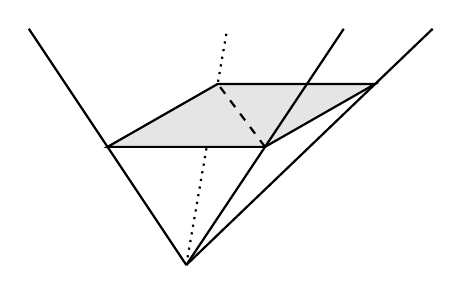
\begin{tikzpicture}
      \draw[thick,dotted] (1,-1.5) -- (1.52,1.5);

      \draw[thick,fill=black!10] (0,0) -- (2,0) -- (3.4,0.8) -- (1.4,0.8) -- cycle;
      \draw[thick,dashed] (2,0) -- (1.4,0.8);

      \draw[thick] (1,-1.5) -- (-1,1.5);
      \draw[thick] (1,-1.5) -- (3,1.5);
      \draw[thick] (1,-1.5) -- (4.13,1.5);
    \end{tikzpicture}
  \end{center}
  \caption{The triangulation of a pointed cone can be obtained from a triangulation of its so-called vertex figure.}
  \label{fig:triangulation-cone}
\end{figure}
\begin{proof}
  Since $C$ is pointed,
  there is an inequality $a^T x \leq 0$ defining its vertex $0$.\footnote{%
  That is, $a^Tx \leq 0$ is valid for $C$ and $a^Tx < 0$ for all $x \in C \setminus \{ 0 \}$.}
  Let $P := C \cap \{ a^Tx = -1 \}$
  and let $\Delta_1, \ldots, \Delta_n$ be its triangulation by Theorem~\ref{thm:polytope-triangulation},
  see Figure~\ref{fig:triangulation-cone}.
  Then the $C_i := \cone \Delta_i$ satisfy the desired properties.
\end{proof}




\section{The algebra of polyhedra}

Given a triangulation of a cone $C$ into simplicial cones $C_1, \ldots, C_n$,
it seems natural to express the generating function $f(C;x)$ as
the sum of the generating functions $f(C_i;x)$.
Note, however, that integer points on lower-dimensional cones that arise from intersections $C_i \cap C_j$
will be counted multiple times.
The generating functions corresponding to those lower dimensional cones must be subtracted,
but then points that have been subtracted too often must be added again, and so on.
In this section, we will put such computations on a rigorous foundation.

\begin{definition}
  We denote
  \begin{enumerate}[(a)]
    \item by $\cP^d$ the set of rational polyhedra in $\R^d$,
    \item by $\cP_0^d \subset \cP^d$ the set of rational polyhedra that contain lines,
    \item by $\cP_v^d \subset \cP^d$ the set of rational polyhedra that do not contain lines
      (i.e., polyhedra with vertices, also known as pointed polyhedra),
    \item by $\cP_b^d \subset \cP^d$ the set of bounded rational polyhedra, and
    \item by $\cP_\ell^d \subset \cP^d$ the set of rational polyhedra that are not full-dimensional.
  \end{enumerate}
\end{definition}
The relationships between those families of polyhedra are as follows:
\begin{center}
  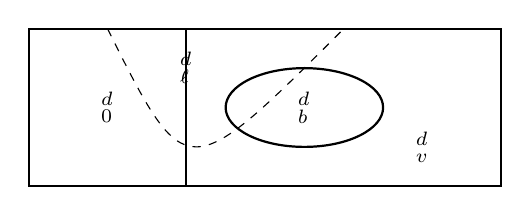
\begin{tikzpicture}
    \draw[thick] (0,0) rectangle (6,2);
    \draw[thick] (2,0) rectangle (2,2);
    \draw (1,1) node {$\cP_0^d$};
    \draw (5,0.5) node {$\cP_v^d$};
    \draw[thick] (3.5,1) ellipse[x radius=1cm,y radius=0.5cm] node {$\cP_b^d$};
    \draw[dashed] (1,2) .. controls (2,0) .. (4,2);
    \draw (2,1.5) node {$\cP_\ell^d$};
  \end{tikzpicture}
\end{center}

\begin{definition}
  Let $P \in \cP^d$.
  The \emph{indicator} or \emph{characteristic} function of $P$ is denoted by $[P] = \chi_P : \R^d \to \R$,
  where
  \[
    [P](x) := \begin{cases}
                1 & x \in P \\
                0 & x \not\in P
              \end{cases}
  \]
  We define $\R \cP^d$ as the sub-vector space of the space of all functions $\R^d \to \R$
  that is generated by $\{ [P] : P \in \cP^d \}$.
  The vector spaces $\R \cP_0^d$ etc. are defined analogously.
\end{definition}

\begin{lemma}[Inclusion-exclusion formula]
  \label{lemma:inclusion-exclusion}
  Let $P_1, \ldots, P_m \in \cP^d$.
  Then
  $[A_1 \cup \dots \cup A_m] = \sum_{\emptyset \neq I \subseteq [m]} (-1)^{|I| - 1} [\bigcap_{i \in I} A_i]$.
\end{lemma}
\begin{proof}
  Left as an exercise.
\end{proof}

\begin{lemma}
  \label{lemma:generating-functions-linear-as-series}
  Let $R := \R[[x_1,\ldots,x_d,x_1^{-1},\ldots,x_d^{-d}]]$ be the vector space of formal power series in $d$ variables.\footnote{%
  This is \emph{not} a ring, because multiplication of formal power series with unbounded positive \emph{and} negative exponents is not defined in general.}
  There exists a unique linear map $F: \R \cP^d \to R$
  such that $F([P]) = f(P;x)$ for all $P \in \cP^d$.
\end{lemma}
\begin{proof}
  If we can show that one such $F$ exists,
  then uniqueness follows immediately because its values are fixed on a generating set of $\R\cP^d$.
  If the $[P]$ for $P \in \cP^d$ were linearly independent,
  then existence of $F$ would be obvious.
  Since they are not, we need to show that our desired values of $F$ are consistent under linear dependencies.

  To be precise, we need to show that for all linear dependencies of the form
  \[
    \sum_{i=1}^n \alpha_i [P_i] = 0
  \]
  one has
  \[
    \sum_{i=1}^n \alpha_i f(P_i; x) = 0,
  \]
  where the equality is in the sense of formal power series.

  The equality of formal power series is defined as the equality of all coefficients.
  That is,
  we need to determine the coefficient $a_p$ of the monomial $x^p$
  for every integer point $p \in \Z^d$.
  In fact,
  \[
    a_p = \sum_{i: p \in P_i} \alpha_i = \left(\sum_{i=1}^n \alpha_i [P_i] \right)(p) = 0 \text{ for all } p \in \Z^d,
  \]
  which completes the proof.
\end{proof}

\begin{corollary}
  \label{corollary:cone-triangulation-series}
  Let $C \in \cP^d$ be a pointed cone with triangulation $C_1, \ldots, C_n \in \cP^d$.
  Then
  \[
    f(C;x) = \sum_{\emptyset \neq I \subseteq [n]} (-1)^{|I| - 1} f(\bigcap_{i \in I} C_i; x)
  \]
  where the equality is understood as equality of formal power series.
\end{corollary}
\begin{proof}
  Follows from Lemmas~\ref{lemma:inclusion-exclusion} and~\ref{lemma:generating-functions-linear-as-series}.
\end{proof}

The sum in Corollary~\ref{corollary:cone-triangulation-series} typically contains
many index sets $I$ for which the intersection $\bigcap_{i \in I} C_i$ is trivial,
i.e., equal to $\{ 0 \}$.
Using tools that we will develop later, it turns out that those summands can be ignored.
Showing this is left as an exercise.

While Lemma~\ref{lemma:generating-functions-linear-as-series}
rigorously justifies computations with power series $f(P;x)$,
we really want an anologous statement for rational functions.
This is not immediate because, as we have seen in Section~\ref{sec:simple-example-generating-functions},
the series $f(P;x)$ converges nowhere for $P \in \cP_0^d$,
and so it is not clear what rational function to assign to such polyhedra.
However, it turns out that assigning rational functions to \emph{pointed} polyhedra is sufficient:

\begin{lemma}
  \label{lemma:algebra-generated-by-pointed}
  $\R \cP^d = \R\cP_v^d$.
\end{lemma}
\begin{proof}
  The inclusion from right to left is immediate.
  We need to show that $[P] \in \R\cP_v^d$ for all $P \in \cP_0^d$;
  the inclusion from left to right then follows by linearity.

  Let $Q_1, \ldots, Q_n \in \cP_v^d$ and $\varepsilon_1, \ldots, \varepsilon_n \in \R$ such that
  \[
    [\R^d] = \sum_{i=1}^n \varepsilon_i [Q_i].
  \]
  One can obtain such an equation by applying the inclusion-exclusion formula to the orthants of $\R^d$.
  We then observe that pointwise multiplication of indicator functions of polyhedra
  corresponds to taking intersections and compute (see Figure~\ref{fig:algebra-generated-by-pointed}):
  \[
    [P] = [\R^d] \cdot [P] = \sum_{i=1}^n \varepsilon_i [Q_i] \cdot [P] = \sum_{i=1}^n \varepsilon_i [Q_i \cap P] \in \R\cP_v^d,
  \]
  since the subset $Q_i \cap P$ of the pointed polyhedron $Q_i$ is pointed as well.
\end{proof}
\begin{figure}
  \begin{center}
    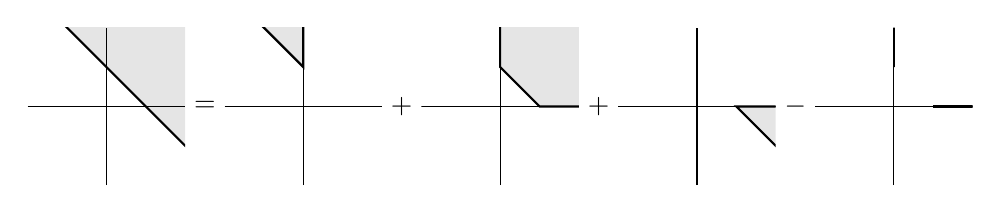
\begin{tikzpicture}
      \begin{scope}
        \clip (-1,-1) rectangle (1,1);

        \draw[thick,fill=black!10] (-1,1.5) -- (1.5,-1) -- (1.5,1.5) -- cycle;
        \draw (-1,0) -- (1,0);
        \draw (0,-1) -- (0,1);
      \end{scope}

      \draw (1.25,0) node {$=$};

      \begin{scope}[xshift=2.5cm]
        \clip (-1,-1) rectangle (1,1);

        \draw[thick,fill=black!10] (-1,1.5) -- (0,0.5) -- (0,1.5) -- cycle;
        \draw (-1,0) -- (1,0);
        \draw (0,-1) -- (0,1);
      \end{scope}

      \draw (3.75,0) node {$+$};

      \begin{scope}[xshift=5cm]
        \clip (-1,-1) rectangle (1,1);

        \draw[thick,fill=black!10] (0,1.5) -- (0,0.5) -- (0.5,0) -- (1.5,0) -- (1.5,1.5) -- cycle;
        \draw (-1,0) -- (1,0);
        \draw (0,-1) -- (0,1);
      \end{scope}

      \draw (6.25,0) node {$+$};

      \begin{scope}[xshift=7.5cm]
        \clip (-1,-1) rectangle (1,1);

        \draw[thick,fill=black!10] (1.5,-1) -- (0.5,0) -- (1.5,0) -- cycle;
        \draw (-1,0) -- (1,0);
        \draw (0,-1) -- (0,1);
      \end{scope}

      \draw (8.75,0) node {$-$};

      \begin{scope}[xshift=10cm]
        \clip (-1,-1) rectangle (1,1);

        \draw[thick,fill=black!10] (0,0.5) -- (0,1) -- cycle;
        \draw[thick,fill=black!10] (0.5,0) -- (1,0) -- cycle;
        \draw (-1,0) -- (1,0);
        \draw (0,-1) -- (0,1);
      \end{scope}
    \end{tikzpicture}%
  \end{center}
  \caption{An illustration of the proof of Lemma~\ref{lemma:algebra-generated-by-pointed}.}
  \label{fig:algebra-generated-by-pointed}
\end{figure}




\section{Rational generating functions of polyhedra}

Let $C = \cone\{u_1,\ldots,u_d\} \in \cP^d$ be a simplicial cone
with $u_j \in \Z^d$ primitive.
Consider the fundamental parallelepiped
\[
  P(C) := \{ \sum_{j=1}^d \lambda_j u_j ~:~ 0\leq \lambda_j < 1 \}
\]
of the cone.
From Chapter~\ref{chapter:basics},
we know that $|P(C) \cap \Z^d| = \det(C)$.

\begin{lemma}
  \label{lemma:series-simplicial-cone}
  $f(C;x) = \left(\sum_{p \in P(C) \cap \Z^d} x^p \right) \prod_{j=1}^d \sum_{n=0}^\infty x^{n u_j}$
  as formal power series.
\end{lemma}
\begin{proof}
  First, observe that the product on the right hand side is well-defined.
  Since the $u_j$ are linearly independent, every $p \in \Z^d$ can be uniquely expressed as a linear combination
  \[
    p = \sum_{j=1}^d \lambda_j u_j
  \]
  and therefore there is at most one choice for $n$ in each of the sums
  so that the corresponding monomials multiply to $x^p$.

  In general, products of monomials correspond to sums of exponents.
  To compare the coefficient of $x^p$ on the left and right hand sides,
  observe that the only possible factorization of $x^p$ on the right hand side is based on
  \[
    p = \sum_{j=1}^d \lfloor \lambda_j \rfloor u_j + \underbrace{\sum_{j=1}^d \{ \lambda_j \} u_j}_{\in P(C) \cap \Z^d}.
  \]
  From this, one can check that the coefficients match.
\end{proof}


\begin{lemma}
  \label{lemma:convergence-simplicial-cone}
  There is an open set $U \subset \C^d$ on which $f(C;x)$ converges absolutely and uniformly on compact subsets.
  Furthermore, $f(C;x) = \left(\sum_{p \in P(C) \cap \Z^d} x^p \right) \frac{1}{\prod_{j=1}^d 1 - x^{u_j}}$
  where the series converges absolutely.
\end{lemma}
\begin{proof}
  Each series $\sum_{n=0}^\infty x^{n u_j}$ is a geometric series
  which converges absolutely and uniformly on compact subsets in the set $\{ x\in \C^d ~:~ |x^{u_j}| < 1 \}$.
  Let $a^T p \leq 0$ be an inequality defining the vertex $0 \in C$;
  that is, $a^T u_j < 0$ for all $j$.
  Let
  \[
    y := (e^{a_1}, \ldots, e^{a_d}) \in \C^d
  \]
  Then all series $\sum_{n=0}^\infty x^{n u_j}$ converge absolutely to $\frac{1}{1 - x^{u_j}}$ on a neighborhood of $y$.
  The convergence is uniform on compact subsets of the neighborhood.
  The desired properties then extend to the series $f(C;x)$ as a whole, because we merely form a finite product with a finite sum.
\end{proof}


We will extend this formula first to general pointed polyhedral cones and then to pointed polyhedra.
First, we make the simple observation that convergence can only get better for generating series
that contain subsets of monomials:

\begin{fact}
  \label{fact:polyhedra-subset-convergence-superset}
  Let $P \subseteq Q$ be polyhedra.
  If $f(Q;x)$ converges absolutely and uniformly on compact subsets on an open set $U \subset \C^d$,
  then so does $f(P;x)$.
\end{fact}

\begin{lemma}
  \label{lemma:series-pointed-converges}
  Let $P \in \cP_v^d$ be a pointed polyhedron.
  Then there is an open set $U \subset \C^d$ on which
  $f(P;x)$ converges absolutely and uniformly on compact subsets.
\end{lemma}
\begin{proof}
  We show that $P$ is contained in a translated simplicial cone,
  so that the result follows from the previous fact combined with Lemma~\ref{lemma:convergence-simplicial-cone}.

  Write $P = \{ p ~:~ Ap \leq b \}$
  and choose a subset of $d$ linearly independent defining inequalities.
  These inequalities define a (translated) simplicial cone $C = \{ p ~:~ A'p \leq b' \}$.
  We can increase the right hand sides $b'$ to obtain a translated cone $C'$
  with integral apex $v \in \Z^d$ and $P \subseteq C \subseteq C'$, see Figure~\ref{fig:series-pointed-converges}.

  Let us write $C' = v + K$ where $K$ is a simplicial cone (with apex $0$).
  It is easy to see that $f(C';x) = x^v f(K;x)$,
  where the equation is understood in terms of formal series.
  Multiplication with a monomial does not change convergence,
  and so the result follows.
\end{proof}
\begin{figure}
  \begin{center}
    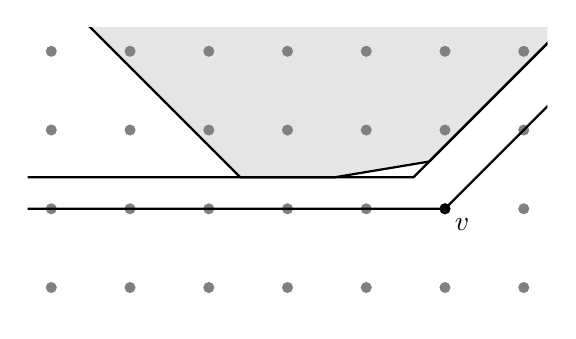
\begin{tikzpicture}
      \clip (-0.3,-0.3) rectangle (6.3,3.3);

      \draw[thick,fill=black!10] (0.3,3.5) -- (2.4,1.4) -- (3.6,1.4) -- (4.8,1.6) -- (6.8,3.6);

      \foreach \x in {0,1,...,6.01}
        \foreach \y in {0,1,...,3.01}
          \fill[black!50] (\x,\y) circle[radius=2pt];

      \draw[thick] (-0.5,1.4) -- (4.6,1.4) -- (6.8,3.6);
      \draw[thick] (-0.5,1.0) -- (5,1.0) -- (8,4);
      \fill[black] (5,1) circle[radius=2pt] node[below right] {$v$};
    \end{tikzpicture}
  \end{center}
  \caption{Every pointed polyhedron is contained in a (translated) simplicial cone with integral apex.}
  \label{fig:series-pointed-converges}
\end{figure}

\begin{lemma}
  \label{lemma:pointed-cone-rational-function}
  Let $C \in \cP_v^d$ be a pointed cone
  with triangulation $C_1 \cup \dots \cup C_n$.
  Let $\hat f_j$ be the rational function associated to $C_j$ by Lemma~\ref{lemma:convergence-simplicial-cone}.
  Then
  \[
    f(C;x) = \sum_{\emptyset \neq I \subseteq [n]} (-1)^{|I| - 1} \hat f_j(x)
  \]
  wherever the series converges absolutely and the rational functions are defined.
\end{lemma}
\begin{proof}
  By Corollary~\ref{corollary:cone-triangulation-series},
  \[
    f(C;x) = \sum_{\emptyset \neq I \subseteq [n]} (-1)^{|I| - 1} f(C_j;x)
  \]
  holds for the formal power series.
  We have $f(C_j;x) = \hat f_j(x)$ where $f(C_j;x)$ converges absolutely,
  and by Fact~\ref{fact:polyhedra-subset-convergence-superset}
  and Lemma~\ref{lemma:series-pointed-converges},
  there is an open set $U \subset \C^d$ where all $f(C_j;x)$ and $f(C;x)$
  converge absolutely and uniformly on compact subsets.
  Hence the statement of the Lemma holds on $U$.
  Since the functions involved are complex differentiable,
  it must hold wherever $f(C;x)$ converges absolutely and the rational functions $\hat f_j$ are defined.
\end{proof}

Now that we have covered all pointed cones,
we can use \emph{homogenization} to extend our results to pointed polyhedra.
Let $P = \{ p \in \R^d ~:~ Ax \leq b \} \in \cP_v^d$ be a pointed polyhedron and define its homogenization
\[
  P' := \{ (p,t) \in \R^{d+1} ~:~ Ax - tb \leq 0, t \geq 0 \}
\]
One easily checks that $P \times \{ 1 \} = P' \cap \{ t = 1\}$, see Figure~\ref{fig:generating-series-homogenization}.
More generally, one has
\[
  P' \cap \{ t = t^\star \} = t^\star P \times \{ t^\star \} \text{ for all } t^\star > 0,
\]
and $P' \cap \{ t = 0 \}$ equals the recession cone of $P$.

\begin{lemma}
  $P'$ is a pointed cone.
\end{lemma}
\begin{proof}
  Clearly, $P'$ is a cone.

  Assume that it is not pointed, that is, it has a non-zero lineality space.
  That is, there is a $(v,\tau) \in \R^{d + 1}$ with $(v,\tau),-(v,\tau) \in P'$.
  The constraint $t \geq 0$ implies $\tau = 0$.
  Plugging this in, we can conclude $Av = 0$.
  However, this means that $v$ lies in the lineality space of $P$,
  which contradicts the assumption that $P$ is pointed.
\end{proof}

\begin{figure}
  \begin{center}
    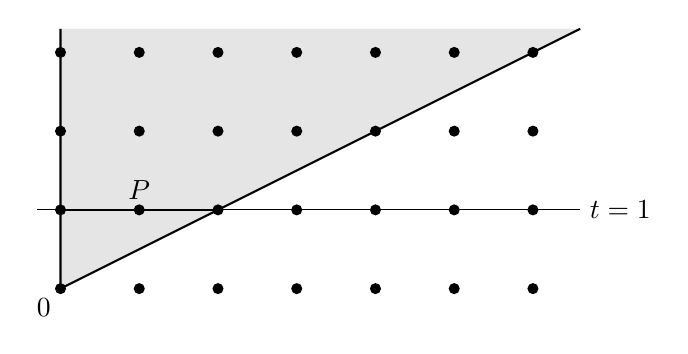
\begin{tikzpicture}
      \draw[thick,fill=black!10] (0,3.3) -- (0,0) -- (6.6,3.3);

      \foreach \x in {0,1,...,6.01}
        \foreach \y in {0,1,...,3.01}
          \fill (\x,\y) circle[radius=2pt];

      \draw (-0.3,1) -- (6.6,1) node[right] {$t = 1$};
      \draw[thick] (0,1) -- node[above] {$P$} (2,1);
      \draw (0,0) node[below left] {$0$};
    \end{tikzpicture}
  \end{center}
  \caption{An example of homogenization.}
  \label{fig:generating-series-homogenization}
\end{figure}

\begin{example}
  Consider the polytope $P = [0,2] \subset \R$ and its homogenization,
  as illustrated in Figure~\ref{fig:generating-series-homogenization}.
  \[
    f(P;x) = 1 + x + x^2
  \]
  and
  \[
    f(P';(x,t)) = 1 + t + tx + tx^2 + t^2 + t^2x + \dots
  \]
  Let us understand the series $f(P';(x,t))$ as a series in $t$ with coefficients in the formal power series $\R[[x,x^{-1}]]$.
  Then we recover $f(P;x)$ as the coefficient of the monomial $t$.
\end{example}

\begin{lemma}
  Let $\hat f$ be the rational function associated to $P'$ by Lemma~\ref{lemma:pointed-cone-rational-function}.
  Then
  $f(P;x) = \left. \frac{d}{dt} \hat f(x,t) \right\rvert_{t = 0}$
  wherever the series converges absolutely.
\end{lemma}
\begin{proof}
  One easily checks that
  \[
    f(P;x) = \left. \frac{d}{dt} f(P';(x,t)) \right\rvert_{t = 0}
  \]
  holds in the sense of symbolic differentiation of formal power series.
  Let us carefully extend the equation to rational functions.

  From the proof of Lemma~\ref{lemma:series-pointed-converges},
  we know that
  \[
    P \subseteq v + C,
  \]
  where $v \in \Z^d$ and $C$ is a simplicial cone.
  Furthermore, we know that there is an open set $U \subset \C^d$
  on which $f(C;x)$ converges absolutely and uniformly on compact subsets.
  We can also give a uniform upper bound $M$ on the sum of absolute values of summands of $f(C;x)$
  for all $x \in U$ (possibly by making $U$ slightly smaller).
  We have
  \[
    P' \cap \{ t = k \} \subseteq (kv + C) \times \{ k \}
  \]
  for all $k \in \N_{\geq 0}$,
  and so we can bound the sum of absolute values of $f(P';(x,t))$ by
  \[
    \sum_{k=0}^\infty M |x^v t|^k
  \]
  for all $x \in U$ and $t \in \C$.
  This sum is finite for $|t| < \frac{1}{|x^v|}$,
  so as long as $U$ is bounded,
  the series $f(P';(x,t))$ converges absolutely and uniformly on compact subsets on $U \times (-t^\star, t^\star)$ for some $t^\star > 0$.

  As a consequence, the formal derivative coincides with the derivative of $\hat f$ on this set,
  and we can evaluate the derivate on $U \times \{ 0 \}$.
  This means that the claim of the Lemma holds on $U$.
  Since the functions involved are complex differentiable,
  the claim extends wherever the series converges absolutely.
\end{proof}

We can now prove an analogue of Lemma~\ref{lemma:generating-functions-linear-as-series}
for rational functions.
We denote the set of rational functions by $\C(x)$
and remind the reader that equality of rational functions is understood to be up to negligible differences
in their domain.

\begin{theorem}
  \label{thm:rational-generating-functions}
  There exists a unique linear map $F: \R\cP^d \to \C(x)$
  such that for all $P \in \R\cP^d$ one has $F([P]) = f(P;x)$ wherever the series converges absolutely.
  This map satisfies
  \begin{enumerate}[(a)]
    \item $F([u + P]) = x^u F([P])$ for all $u \in \Z^d$ and
    \item $F([P]) = 0$ for all $P \in \cP_0^d$.
  \end{enumerate}
\end{theorem}
\begin{proof}
  By the previous sequence of Lemmas, we have candidate rational functions $f_P$
  for every $P \in \cP_v^d$.
  By Lemma~\ref{lemma:algebra-generated-by-pointed},
  this is sufficient to ensure that $F$ is unique if it exists.
  To show that our candidate rational functions give rise to a linear map $F$,
  we have to show that they are consistent with linear dependencies.
  That is, whenever we have $P_1,\ldots,P_m \in \cP_v^d$ and $\alpha_1,\ldots,\alpha_m \in \R$ with
  \[
    \sum_j \alpha_j [P_j] = 0
  \]
  we must have
  \[
    \sum_j \alpha_j f_{P_j} = 0.
  \]
  Lemma~\ref{lemma:generating-functions-linear-as-series} implies that
  \[
    \sum_j \alpha_j f(P_j;x) = 0
  \]
  holds in the sense of formal power series,
  so we are done immediately if the $f(P_j;x)$ have a common region of absolute convergence.
  However, this is not the case in general.

  As in the proof of Lemma~\ref{lemma:algebra-generated-by-pointed},
  let $Q_1, \ldots, Q_n \in \cP_v^d$ and $\varepsilon_1, \ldots, \varepsilon_n \in \R$ such that
  \[
    [\R^d] = \sum_{i=1}^n \varepsilon_i [Q_i].
  \]
  Fix a $Q_i$. Pointwise multiplication by $Q_i$ tells us that
  \[
    \sum_j \alpha_j [P_j \cap Q_i] = 0,
  \]
  and since the $P_j \cap Q_i \subseteq Q_i$ have a common region of absolute convergence,
  we get
  \[
    \sum_j \alpha_j f_{P_j \cap Q_i} = 0.
  \]
  Similarly, we can fix a $P_j$ and get
  \[
    [P_j] = \sum_{i=1}^n \varepsilon_i [P_j \cap Q_i].
  \]
  Since $P_j$ is pointed, all the $P_j \cap Q_i$ have a common region of absolute convergence
  and we get
  \[
    f_{P_j} = \sum_{i=1}^n \varepsilon_i f_{P_j \cap Q_i}.
  \]
  Putting things together, we can compute
  \begin{align*}
    \sum_j \alpha_j f_{P_j}
     &= \sum_j \alpha_j \sum_{i=1}^n \varepsilon_i f_{P_j \cap Q_i} \\
     &= \sum_{i=1}^n \varepsilon_i \underbrace{\sum_j \alpha_j f_{P_j \cap Q_i}}_{=0} = 0,
  \end{align*}
  which shows that our choice of $f_{P_j}$ can indeed be extended to a linear map $F$.

  Let $P \in \cP_v^d$ and let $u \in \Z^d$.
  One easily verifies that
  \[
    f(u+P;x) = x^u f(P;x)
  \]
  holds in the sense of formal power series.
  The series share a region of absolute convergence, and so
  \[
    F([u + P]) = x^u F([P])
  \]
  holds for pointed polyhedra.
  Since the pointed polyhedra generate all of $\R\cP^d$,
  the equation holds for all polyhedra by linear extension.

  Let $P \in \cP_0^d$. Since $P$ is rational, there is a vector $u \in \Z^d \cap L(P)$; that is, $P = u + P$.
  Using the previous result, we compute
  \[
    F([P]) = F([u + P]) = x^u F([P]),
  \]
  from which we conclude $F([P]) = 0$.
\end{proof}

Theorem~\ref{thm:rational-generating-functions} completely resolves
the problems that were discussed at the end of Section~\ref{sec:simple-example-generating-functions}.

At this point, we already have tools to obtain rational generating functions for polytopes.
However, there are still some weaknesses, in particular:
\begin{enumerate}
  \item Correctly triangulating a cone involves setting up a linear combination with many lower dimensional cones.

  \item The size of the generating function of a simplicial cone $C$ is proportional to $\det C$,
    which can be exponentially large.
\end{enumerate}
We will address these issues in the next sections.




\section{The Euler characteristic and the polarity trick}

The main surprise of this section is that taking polars is a linear operation
as far as the algebra of polyhedra is concerned.
That is, if
\[
  \sum_i \alpha_i [P_i] = 0,
\]
then
\[
  \sum_i \alpha_i [P_i^\star] = 0
\]
holds as well.
This leads to a useful alternative approach for decomposing a cone $C$,
the so-called \emph{polarity trick}:
\begin{enumerate}
  \item Decompose $C^\star$ into pointed cones $C_j$, including lower-dimensional cones.

  \item Take the polar of this decomposition.
    Lower-dimensional cones $C_j$ turn into cones $C_j^\star$ that contain lines.
    Their rational generating function is $0$.
\end{enumerate}
This way, we do not have to keep track of lower-dimensional cones during the decomposition.
To obtain this result, we use a powerful tool that is quite surprising in its own right.

\begin{lemma}[Euler characteristic]
  \label{lemma:euler-characteristic}
  There exists a unique linear map $\mu: \R\cP^d \to \R$
  with $\mu([P]) = 1$ for all non-empty polyhedra $P \in \cP^d$.
\end{lemma}

Before we look at the proof,
take a moment to appreciate some consequences of the existence of this map.
Say we triangulated a polytope $P$ into simplices $\Delta_1, \ldots, \Delta_n$.
Inclusion-exclusion tells us that
\[
  [P] = \sum_{\emptyset \neq I \subseteq [n]} (-1)^{|I| - 1} [\bigcap_{i \in I} \Delta_i],
\]
and it is a simple matter of the binomial formula that the coefficients in the sum on the right-hand-side sum up to $1$.
What the Euler characteristic tells us is that we \emph{also} obtain $1$
if we only sum up the coefficients for sets $I$
where the intersection $\bigcap_{i \in I} \Delta_i$ is non-empty.
This is by no means obvious.

Some additional non-trivial consequences
including the Euler formula for polyhedra
are found in the exercises.

\begin{figure}
  \begin{center}
  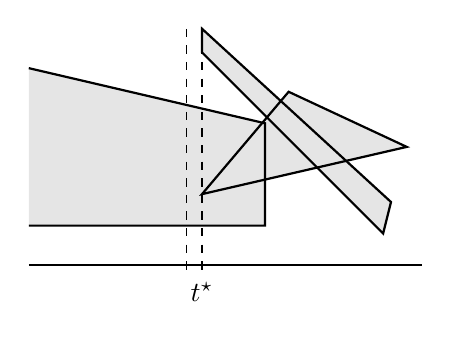
\begin{tikzpicture}
    \draw (0,0) -- (5,0);

    \fill[black!10] (0,0.5) -- (3,0.5) -- (3,1.8) -- (0,2.5);
    \fill[black!10] (2.2,0.9) -- (4.8,1.5) -- (3.3,2.2) -- cycle;
    \fill[black!10] (2.2,3.0) -- (2.2,2.7) -- (4.5,0.4) -- (4.6,0.8) -- cycle;

    \draw[thick] (0,0.5) -- (3,0.5) -- (3,1.8) -- (0,2.5);
    \draw[thick] (2.2,0.9) -- (4.8,1.5) -- (3.3,2.2) -- cycle;
    \draw[thick] (2.2,3.0) -- (2.2,2.7) -- (4.5,0.4) -- (4.6,0.8) -- cycle;

    \draw[dashed] (2.2,3.0) -- (2.2,-0.1) node[below] {$t^\star$};
    \draw[dashed] (2.0,3.0) -- (2.0,-0.1);
  \end{tikzpicture}
  \end{center}
  \caption{An illustration of the proof of Lemma~\ref{lemma:euler-characteristic}.}
  \label{fig:proof-euler-characteristic}
\end{figure}
\begin{proof}
  Again, uniqueness is immediate if we can show existence.
  To show existence, we need to show that whenever
  \[
    \sum_i \alpha_i [P_i] = 0
  \]
  for some non-empty polyhedra $P_1, \ldots, P_n \in \cP^d$ and $\alpha_i \in \R$,
  we have
  \[
    \sum_i \alpha_i = 0.
  \]
  This follows immediately if the $P_i$ share one point in common.
  In particular, it holds when $d = 0$.
  For the general case, we proceed by induction on $d$.
  Since the result holds for $d = 0$, let $d \geq 1$.

  Let $\pi : \R^d \to \R$ be a linear projection (e.g. onto the first coordinate).
  For $t \in \R$, let
  \[
    \sigma(t) := \sum_{i : t \in \pi(P_i)} \alpha_i.
  \]
  Observe that
  \[
    \sigma(t) = \sum_i \alpha_i \mu([P_i \cap \pi^{-1}(t)])
      = \mu\big( \underbrace{\sum_i \alpha_i [P_i \cap \pi^{-1}(t)]}_{=0} \big)
      = 0
  \]
  by the induction hypothesis.
  As $t$ travels along $\R$,
  the summands in the definition of $\sigma(t)$ change,
  yet $\sigma(t)$ stays the same, see Figure~\ref{fig:proof-euler-characteristic}.
  This allows us to partition the $\alpha_i$ into sets based on the point in time when they enter the definition of $\sigma(t)$.
  Formally, let
  \[
     t_i := \min\pi(P_i) \in \R \cup \{ -\infty \}
  \]
  For $t$ sufficiently small,
  we get
  \[
    0 = \sigma(t) = \sum_{i : t_i = -\infty} \alpha_i.
  \]
  For $t^\star \in \R$, we get
  \[
    0 = \sigma(t^\star) - \lim_{\varepsilon \to 0+} \sigma(t^\star - \varepsilon) = \sum_{i: t_i = t^\star} \alpha_i.
  \]
  Overall, we obtain
  \[
    \sum_i \alpha_i = \underbrace{\sum_{i : t_i = -\infty} \alpha_i}_{=0} + \sum_{t^\star \in \R} \underbrace{\sum_{i: t_i = t^\star} \alpha_i}_{=0} = 0 \qedhere
  \]
\end{proof}



\begin{lemma}[Polarity is linear]
  \label{lemma:polarity-is-linear}
  There is a unique linear map $\cD: \R\cP^d \to \R\cP^d$
  with $\cD([P]) = [P^\star]$ for all $P \in \cP^d$.
\end{lemma}
\begin{figure}
  \begin{center}
    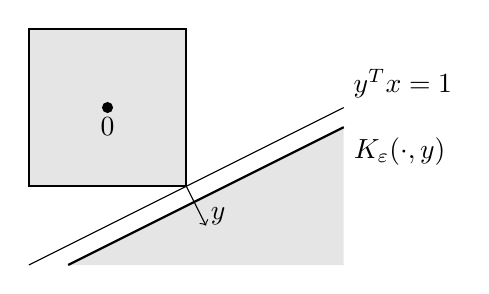
\begin{tikzpicture}
      \draw[thick,fill=black!10] (-1,-1) -- (1,-1) -- (1,1) -- (-1,1) -- cycle;
      \fill (0,0) circle[radius=2pt] node[below] {$0$};

      \draw (-1,-2) -- (3,0) node[above right] {$y^Tx = 1$};

      \fill[black!10] (-.5,-2) -- (3,-.25) -- (3,-2) -- cycle;
      \draw[thick] (-.5,-2) -- (3,-.25) node[below right] {$K_\varepsilon(\cdot, y)$};

      \draw[->] (1,-1) -- node[right, near end] {$y$} +(.25,-.5);
    \end{tikzpicture}
  \end{center}
  \caption{The proof of Lemma~\ref{lemma:polarity-is-linear}. $\mu(K_0(\cdot, y)\cdot [P]) = 1$,
    but the limit is $0$.}
  \label{fig:proof-polarity-is-linear}
\end{figure}
\begin{proof}
  We use the \emph{kernel map}
  \[
    K_\varepsilon(x,y) := \begin{cases}
                1 & y^Tx \geq 1 + \varepsilon \\
                0 & y^Tx < 1 + \varepsilon
              \end{cases}
  \]
  for $\varepsilon > 0$ to define
  \[
    \cD(f)(y) := \mu(f) - \lim_{\varepsilon \to 0} \mu(K_\varepsilon(\cdot, y) \cdot f).
  \]
  For a fixed $y \in \R^d$,
  the map $K_\varepsilon(\cdot, y): \R^d \to \R$ is the indicator function
  of the half-space $\{ x \in \R^d ~:~ y^Tx \geq 1 + \varepsilon\}$,
  and $K_\varepsilon(\cdot, y) \cdot f$ is simply point-wise multiplication.
  See Figure~\ref{fig:proof-polarity-is-linear} for an illustration.

  To see that the definition of $\cD$ makes sense,
  we need to verify that the limit exists.
  Choose an arbitrary representation
  \[
    f = \sum_i \alpha_i [P_i]
  \]
  with $P_i \in \cP^d$.
  We can compute
  \begin{align*}
    \lim_{\varepsilon \to 0} \mu(K_\varepsilon(\cdot, y) \cdot f)
      &= \sum_i \alpha_i \cdot \lim_{\varepsilon \to 0} \mu(K_\varepsilon(\cdot, y) \cdot [P_i]) \\
      &= \sum_i \alpha_i \cdot \lim_{\varepsilon \to 0} \mu([P_i \cap \{ x ~:~ y^Tx \geq 1 + \varepsilon \}])
  \end{align*}
  The term $\mu([P_i \cap \{ x ~:~ y^Tx \geq 1 + \varepsilon \}])$ is either $0$ or $1$,
  and it is monotonically increasing as $\varepsilon$ goes to $0$ from above, so the limit exists.

  In fact, if $f = [P]$ for some polyhedron $P \in \cP^d$,
  the limit is equal to $1$ if and only if $y^Tx > 1$ for some $x \in P$.
  It follows that
  \[
    \cD([P]) = [P^\star].
  \]
  One easily verifies that $\cD(f)(y)$ is linear in $f$, and therefore $\cD$ is linear.
  By linearity, it also follows that $\cD(f) \in \R\cP^d$ for all $f \in \R\cP^d$.
  As usual, uniqueness follows because the value of the desired map $\cD$ is fixed on a generating set of $\R\cP^d$.
\end{proof}





\section{Signed decomposition into unimodular cones}

Recall that our candidate rational generating function for a simplicial cone
$C = \cone\{u_1, \ldots, u_d \}$ with $u_j \in \Z^d$ primitive is
\[
  f(C;x) = \left(\sum_{p \in P(C) \cap \Z^d} x^p \right) \frac{1}{\prod_{j=1}^d 1 - x^{u_j}},
\]
where the fundamental parallelepiped $P(C)$ of $C$ may contain exponentially many integer points
in the encoding length of $C$.
This is clearly wasteful, so we would like to decompose $C$ into unimodular cones.

Every cone can be triangulated into finitely many unimodular cones (showing this is left as an exercise),
but doing so may be wasteful as well.
Consider the cone
\[
  C := \cone\{ \underbrace{\begin{pmatrix} 0 \\ 1 \end{pmatrix}}_{=: u_1}, \underbrace{\begin{pmatrix} N \\ 1 \end{pmatrix}}_{=: u_2} \},
\]
see Figure~\ref{fig:cone-bad-unimodular-triangulation}.
The reader may convince themselves that any unimodular cone contained in $C$
covers at most one unit of length on the line segment between $u_1$ and $u_2$.
Hence at least $N$ unimodular cones are required in any unimodular triangulation,
which is an exponential number in the encoding length of $C$.
\begin{figure}
  \begin{center}
    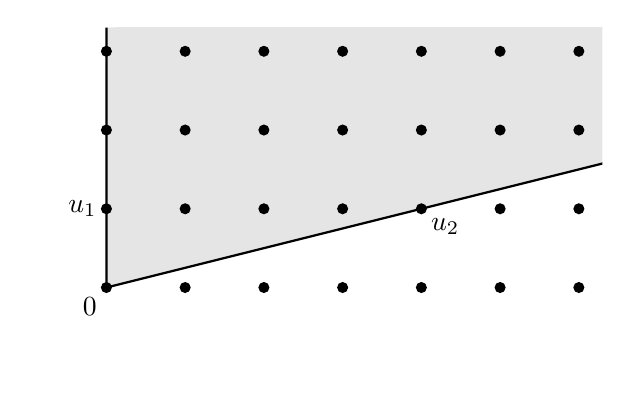
\begin{tikzpicture}
      \clip (-1,-1) rectangle (6.3,3.3);

      \draw[thick,fill=black!10] (0,3.3) -- (0,0) -- (16,4);

      \foreach \x in {0,1,...,6.01}
        \foreach \y in {0,1,...,3.01}
          \fill[black] (\x,\y) circle[radius=2pt];

      \draw (0,0) node[below left] {$0$};
      \draw (0,1) node[left] {$u_1$};
      \draw (4,1) node[below right] {$u_2$};
    \end{tikzpicture}
  \end{center}
  \caption{Every unimodular triangulation requires at least $N$ cones.}
  \label{fig:cone-bad-unimodular-triangulation}
\end{figure}

On the other hand,
the cones $C_1 = \cone\{ e_1, e_2 \}$ and $C_2 = \cone\{ e_1, u_2 \}$ are both unimodular
and we can write
\[
  [C] \equiv [C_1] - [C_2] \pmod{\R\cP_\ell^d},
\]
where we ignore lower-dimensional cones because they will ultimately be irrelevant thanks to the polarity trick.
We will show that this idea can be generalized.

\begin{lemma}
  \label{lemma:simplicial-cone-signed-star}
  Let $C = \cone\{u_1,\ldots,u_d\}$ be a simplicial cone and let
  $v = \sum_{j=1}^d \lambda_j u_j$ be a vector with at least one $\lambda_j > 0$.
  Then
  \[
    [C] \equiv \sum_{j=1}^d \sgn \lambda_j [C_j] \pmod{\R\cP_\ell^d},
  \]
  where $C_j = \cone\{u_1,\ldots,v,\ldots,u_d\}$ is the simplicial cone obtained by
  replacing $u_j$ by $v$.
\end{lemma}
\begin{proof}
  Left as an exercise.
\end{proof}

Observe that if one of the $\lambda_j = 0$,
the number of cones in the decomposition is less than $d$.
This is intuitively plausible because in this situation,
$v$ lies in one of the facets of $C$.

\begin{lemma}
  \label{lemma:signed-decomposition-determinants}
  Let $C \in \R\cP^d$ be a simplicial cone with $\det C \geq 2$.
  There exists a signed decomposition
  \[
    [C] \equiv \sum_{j=1}^d \varepsilon_j [C_j] \pmod{\R\cP_\ell^d},
  \]
  with $\varepsilon_j = \pm1$ such that $\det C_j \leq (\det C)^{1-1/d}$.

  If $d$ is fixed, such a decomposition can be computed in polynomial time.
\end{lemma}
\begin{figure}
  \begin{center}
    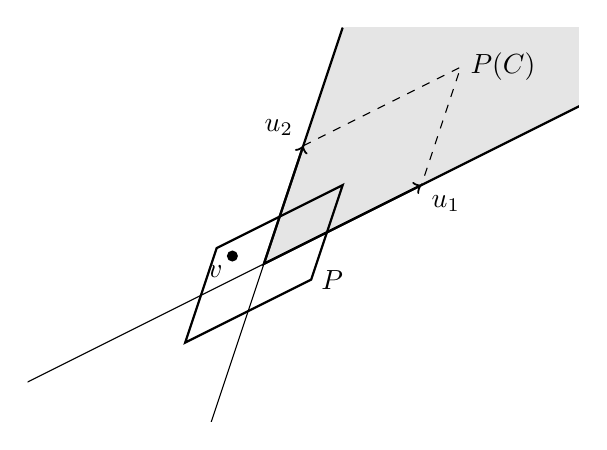
\begin{tikzpicture}
      \clip (-3,-2) rectangle (4,3);

      \draw (-4,-2) -- (4,2);
      \draw (-1,-3) -- (1,3);
      \draw[thick,fill=black!10] (1,3) -- (0,0) -- (8,4);
      \draw[thick,->] (0,0) -- (2,1) node[below right] {$u_1$};
      \draw[thick,->] (0,0) -- (.5,1.5) node[above left] {$u_2$};
      \draw[dashed] (.5,1.5) -- (2.5,2.5) node[right] {$P(C)$} -- (2,1);

      \draw[thick] (1,1) -- ++(-.4,-1.2) node[right] {$P$} -- ++(-1.6,-.8) -- ++(.4,1.2) -- cycle;

      \fill (-.4,.1) circle[radius=2pt] node[below left] {$v$};
    \end{tikzpicture}
  \end{center}
  \caption{To obtain a good decomposition of a simplicial cone,
    we find integer vectors in a scaling of the fundamental parallelepiped.}
  \label{fig:signed-decomposition-determinants}
\end{figure}
\begin{proof}
  Let $C = \cone\{ u_1, \ldots, u_d \}$ with $u_j \in \Z^d$ primitive.
  We will make use of the signed decomposition of Lemma~\ref{lemma:simplicial-cone-signed-star}.
  Given
  \[
    v = \sum_j \lambda_j u_j \in \Z^d,
  \]
  the cone $C_j = \cone\{u_1,\ldots,v,\ldots,u_d\}$ has determinant
  \[
    \det C_j = |\lambda_j| \det C.
  \]
  To see this, recall that $\det C$ is the volume of the fundamental parallelepiped $P(C)$ spanned by the $u_j$.
  Replacing $u_j$ by $v$ multiplies the height of $P(C)$ above the facet spanned by $u_i$, $i \neq j$,
  by a factor of $\lambda_j$, and hence we get the desired relation for the volume and determinants.

  Given that $\det C \geq 2$, there is a non-zero integer vector in $P(C)$.
  However, we cannot guarantee that its coefficients in the basis of the $u_j$ are sufficiently small.
  So let us symmetrize and scale $P(C)$ to obtain the compact parallelepiped
  \[
    P := \{ \sum_j \lambda_j u_j ~:~ |\lambda_j| \leq (\det C)^{-1/d} \},
  \]
  see Figure~\ref{fig:signed-decomposition-determinants}.
  Its volume is
  \[
    \vol(P) = 2^d (\det C)^{-1} \vol P(C) = 2^d,
  \]
  so $P$ contains a non-zero integer vector $v$ by Minkowski's theorem.
  Without loss of generality,
  \[
    v = \sum_j \lambda_j u_j
  \]
  with at least one $\lambda_j > 0$ (otherwise take $-v$).
  We get the desired decomposition by Lemma~\ref{lemma:simplicial-cone-signed-star},
  and
  \[
    \det C_j = |\lambda_j| \det C \leq (\det C)^{1-1/d}.
  \]
  Finding $v$ is a shortest vector problem in a linearly distorted $\ell_\infty$-norm.
  If $d$ is fixed, this can be done in polynomial time.
\end{proof}

Let us now decompose simplicial cones recursively.
We obtain a rooted tree of cones
with outdegrees bounded by $d$:
\begin{center}
  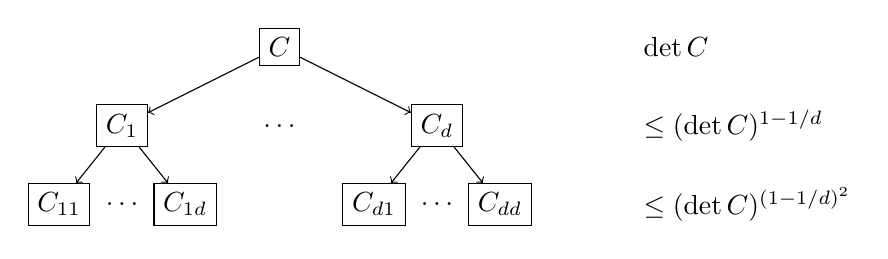
\begin{tikzpicture}
    \node[draw] (r) at (0,0) {$C$};
    \node[right] at (4.5,0) {$\det C$};

    \node[draw] (c1) at (-2,-1) {$C_1$};
    \node at (0,-1) {$\dots$};
    \node[draw] (cd) at (2,-1) {$C_d$};
    \node[right] at (4.5,-1) {$\leq (\det C)^{1-1/d}$};

    \draw[->] (r) -- (c1);
    \draw[->] (r) -- (cd);

    \node[draw] (c11) at (-2.8,-2) {$C_{11}$};
    \node at (-2,-2) {$\dots$};
    \node[draw] (c1d) at (-1.2,-2) {$C_{1d}$};
    \node[draw] (cd1) at (1.2,-2) {$C_{d1}$};
    \node at (2,-2) {$\dots$};
    \node[draw] (cdd) at (2.8,-2) {$C_{dd}$};
    \node[right] at (4.5,-2) {$\leq (\det C)^{(1-1/d)^2}$};

    \draw[->] (c1) -- (c11);
    \draw[->] (c1) -- (c1d);
    \draw[->] (cd) -- (cd1);
    \draw[->] (cd) -- (cdd);
  \end{tikzpicture}
\end{center}
The unimodular cones that appear in the final decomposition correspond exactly to the leaves of the tree.
Let us bound their number.
At level $k$, the determinant of each cone is at most $(\det C)^{(1-1/d)^k}$.
Let us say that the tree goes down to level $\ell + 1$.
Then there must be at least one cone of determinant $\geq 2$ at level $\ell$:
\[
  2 \leq (\det C)^{(1 - 1/d)^\ell}.
\]
Taking logarithms, we get
\[
  1 \leq (1 - 1/d)^\ell \log\det C.
\]
Taking logarithms again, we get
\[
  0 \leq \ell \log(1 - 1/d) + \log\log\det C.
\]
Using $\ln(1 + x) \leq x$, we get
\[
  \ell \leq d \ln 2 \cdot \log\log\det C.
\]
Since every node of the tree has at most $d$ children,
the number of leaves of the tree is bounded by
\[
  d^{\ell + 1} = d \cdot d^{d \ln 2 \cdot \log\log\det C} \leq d \cdot (\log\det C)^{d \ln d}.
\]
Since $\log\det C$ is a polynomial in the encoding length of $C$,
the overall number of unimodular cones in the decomposition is polynomial if $d$ is fixed.

Let us now bound the encoding lengths of the resulting unimodular cones
by bounding the lengths of their generating vectors.\footnote{%
Alternatively, one might want to represent the cones using linear systems of the form $Ax \leq 0$.
The two representations are polynomially related to each other via linear algebra.}
A conservative bound of the vector $v$ that is constructed in the proof of Lemma~\ref{lemma:signed-decomposition-determinants} is
\[
  \|v\|_\infty \leq d\cdot \max_j \|u_j\|_\infty.
\]
With $M := \max_j \|u_j\|_\infty$ where the $u_j$ are the generators of the initial cone $C$,
the $\ell_\infty$-norm of generating vectors at level $k$ of the tree are bounded by $d^k M$.
That is, the encoding lengths of components of the generators of the final unimodular cones are bounded by
\[
  \log d^{\ell + 1} M = (1 + d \ln 2 \cdot \log\log\det C) \cdot \log d + \log M,
\]
which is polynomial in the encoding length of the original cone.

\begin{theorem}
  \label{thm:cone-decomposition}
  For every full-dimensional cone $C \in \cP_v^d$
  there is a set $C_1, \ldots, C_n$ of unimodular cones
  and $\varepsilon_1, \ldots, \varepsilon_n$ such that
  \[
    [C] = \sum_{i=1}^n \varepsilon_i [C_i] \pmod{\R\cP_\ell^d}
  \]
  If $d$ is fixed, this decomposition can be computed in polynomial time.
\end{theorem}
\begin{proof}
  Combine the preceding discussion with the triangulation into simplicial cones of Corollary~\ref{corollary:cone-triangulation}.
\end{proof}

\begin{corollary}
  \label{corollary:cone-decomposition}
  For every cone $C \in \cP_v^d$
  there is a set $C_1, \ldots, C_n$ of unimodular cones
  and $\varepsilon_1, \ldots, \varepsilon_n$ such that
  \[
    f(C;x) = \sum_{i=1}^n \varepsilon_i f(C_i;x)
  \]
  If $d$ is fixed, this decomposition can be computed in polynomial time.
\end{corollary}
\begin{proof}
  We use the polarity trick:
  Apply Theorem~\ref{thm:cone-decomposition} to $C^\star$.
  Then polarize the resoluting decomposition to get an equation of indicator functions modulo $\R\cP_0^d$
  and use the fact that the rational generating functions for polyhedra with lines are $0$.
  Observe that the polar of a unimodular cone is again a unimodular cone.
\end{proof}






\section{Convolution and Brion's theorem}

We will show one more surprising result about the algebra of polyhedra
that generalizes an observation we have made at the end of Section~\ref{sec:simple-example-generating-functions}.

\begin{definition}
  Let $P \in \cP^d$ and let $x \in \R^d$.
  The \emph{tangent cone} of $P$ at $x$ is the set
  \[
    \tcone(P,x) := x + \{ v \in \R^d ~:~ \exists \varepsilon > 0:~ x + \varepsilon v \in P \}
  \]
\end{definition}

The tangent cone is not actually cone, but it is a translate of a cone.
Note that it is defined for all $x$,
but we are mostly interested in the case where $x$ is a vertex, see Figure~\ref{fig:tangent-cone}.
\begin{figure}
  \begin{center}
    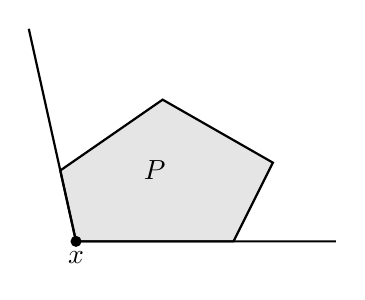
\begin{tikzpicture}
      \draw[thick,fill=black!10] (0,0) -- (2,0) -- (2.5,1) -- (1.1,1.8) -- (-0.2,0.9) -- cycle;
      \node at (1,0.9) {$P$};

      \fill (0,0) circle[radius=2pt] node[below] {$x$};

      \draw[thick] (-0.6,2.7) -- (0,0) -- (3.3,0);
    \end{tikzpicture}
  \end{center}
  \caption{The tangent cone of $P$ at $x$.}
  \label{fig:tangent-cone}
\end{figure}
The main result of this section will be:

\begin{theorem}[Brion]
  \label{thm:brion}
  Let $P \in \cP^d$ and let $V$ be the set of vertices of $P$.
  Then
  \[
    [P] \equiv \sum_{x \in V} [\tcone(P,x)] \pmod{\R\cP_0^d}
  \]
\end{theorem}

Note that we could also write
\[
  [P] \equiv \sum_{x \in \R^d} [\tcone(P,x)] \pmod{\R\cP_0^d}
\]
because $[\tcone(P,x)] \equiv 0 \pmod{\R\cP_0^d}$ when $x$ is not a vertex of $P$.
Before we can proceed with the proof,
we need to develop some more algebraic tools that are of independent interest.

\begin{lemma}
  \label{lemma:polyhedra-affine}
  Let $A : \R^m \to \R^n$ be an affine map.
  There is a unique linear map $\cA: \R\cP^m \to \R\cP^n$
  that satisfies $\cA([P]) = [AP]$ for all $P \in \cP^m$.
\end{lemma}
\begin{proof}
  The proof is analogous to the proof of Lemma~\ref{lemma:polarity-is-linear} that polarity is linear.
  Using the kernel function
  \[
    K(x,y) := \begin{cases} 1 & Ax = y \\ 0 & Ax \neq y \end{cases}
  \]
  we define
  \[
    \cA(f)(y) := \mu(K(\cdot, y) \cdot f).
  \]
  The function $\cA$ is linear because $\cA(f)(y)$ is linear in $f$ for all $y$.
  Since $K(\cdot,y)$ is the indicator function of the preimage of $y$ under $A$,
  we get
  \[
    \cA([P]) = [AP]
  \]
  from the fact that $\mu(K(\cdot, y) \cdot [P]) = 1$ if and only if the preimage of $y$ under $A$ intersects $P$.
  By linearity, it follows that $\cA(f) \in \R\cP^n$ for all $f \in \R\cP^m$.
  As usual, uniqueness follows because the value of the desired map $\cA$ is fixed on a generating set of $\R\cP^m$.
\end{proof}

\begin{lemma}[Convolution]
  \label{lemma:polyhedra-convolution}
  There is a unique bilinear map $\star: \R\cP^d \times \R\cP^d \to \R\cP^d$
  that satisfies $[P] \star [Q] = [P + Q]$ for all $P, Q \in \cP^d$.
\end{lemma}
\begin{proof}
  We define $\star$ as a composition
  \[
    \star: \R\cP^d \times \R\cP^d \stackrel{\times}{\longrightarrow} \R\cP^{d+d} \stackrel{\cA}{\longrightarrow} \R\cP^d
  \]
  where
  \[
    (f \times g)(x,y) := f(x) \cdot g(y)
  \]
  for all $(f,g) \in \R\cP^d \times \R\cP^d$
  and $\cA$ is the lifting of the linear map
  \[
    A(x,y) := x + y
  \]
  due to Lemma~\ref{lemma:polyhedra-affine}.
  Note that $\times$ is well-defined since given
  \[
    f = \sum_i \alpha_i [P_i] \quad\text{ and }\quad g = \sum_j \beta_j [Q_j]
  \]
  one has
  \[
    f \times g = \sum_i \sum_j \alpha_i \beta_j [P_i \times Q_j],
  \]
  that is, $f\times g \in \R\cP^{d+d}$.
  In particular,
  \[
    [P] \times [Q] = [P \times Q]
  \]
  and therefore
  \[
    [P] \star [Q] = [P + Q]
  \]
  as desired.

  Since $\times$ is bilinear and $\cA$ is linear, $\star$ is bilinear.
  It is the unique bilinear map with the desired property
  since its value on a generating system is fixed.
\end{proof}

\begin{proof}[Proof of Theorem~\ref{thm:brion}]
  Observe that the result is trivially true when $P$ contains lines,
  so we can restrict our attention to pointed polyhedra.

  Let us first consider the case of a full-dimensional simplex $\Delta$.
  We can write
  \[
    \Delta = H_0 \cap H_1 \cap \dots \cap H_d
  \]
  where the $H_j$ are closed half-spaces, see Figure~\ref{fig:brion-simplex}.
\begin{figure}
  \begin{center}
    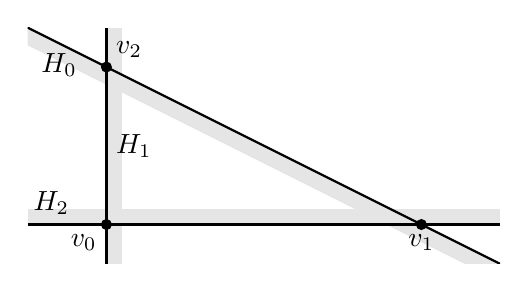
\begin{tikzpicture}
      \clip (0,0) rectangle (6,3);

      \fill[black!10] (0,0.5) -- ++(6,0) -- ++(0,0.2) -- ++(-6,0) -- cycle;
      \fill[black!10] (1,0) -- ++(0,3) -- ++(0.2,0) -- ++(0,-3) -- cycle;
      \fill[black!10] (-2,4) -- ++(8,-4) -- ++(-.09,-.18) --++(-8,4) -- cycle;
      \draw[thick] (0,0.5) -- ++(6,0);
      \draw[thick] (1,0) -- ++(0,3);
      \draw[thick] (-2,4) -- ++(8,-4);

      \coordinate (v0) at (1,0.5);
      \coordinate (v1) at (5,0.5);
      \coordinate (v2) at (1,2.5);

      \fill (v0) circle[radius=2pt] node[below left] {$v_0$};
      \fill (v1) circle[radius=2pt] node[below] {$v_1$};
      \fill (v2) circle[radius=2pt] node[above right] {$v_2$};

      \node[below] at (0.4,2.8) {$H_0$};
      \node[above] at (0.3,0.5) {$H_2$};
      \node[right] at (1,1.5) {$H_1$};
    \end{tikzpicture}
  \end{center}
  \caption{A simplex is the intersection of half-spaces $H_j$.}
  \label{fig:brion-simplex}
\end{figure}
  We write $v_j$ for the vertex opposite to the facet defined by $H_j$.
  By the inclusion-exclusion principle,
  \[
    [\R^d] = \sum_{\emptyset \neq I \subseteq \{0,\ldots,d\}} (-1)^{|I| - 1} [\bigcap_{i\in I} H_i].
  \]
  Analyzing the individual intersections,
  we find that for $I = \{0,\ldots,d\} \setminus \{ j \}$ we have
  \[
    \bigcap_{i \in I} H_i = \tcone(\Delta, v_j)
  \]
  and
  \[
    [\bigcap_{i \in I} H_i] \equiv 0 \pmod{\R\cP_0^d}
  \]
  for $|I| < d$.
  Rearranging terms, we get
  \[
    [\Delta] \equiv \sum_{j=0}^{d} [\tcone(\Delta, v_j)] \pmod{\R\cP_0^d}.
  \]
  The same result follows for lower-dimensional simplices,
  either by considering them in their affine hull or by adding an intersection with the affine hull of $\Delta$
  everywhere in the argument above.

  Now let $P = \conv\{ u_1, \ldots, u_n \}$ be a rational polytope.
  Consider the simplex $\Delta := \conv\{ e_1, \ldots, e_n \} \subset \R^n$
  and the linear map $A: \R^n \to \R^d$ defined by
  \[
    A(e_j) := u_j.
  \]
  Clearly, $A(\Delta) = P$.
  Furthermore, we claim that $A(\tcone(\Delta, e_j)) = \tcone(P, u_j)$.
  This follows from the fact that
  \[
    \tcone(\Delta, e_j) = e_j + \cone\{ e_1 - e_j,  \ldots, e_n - e_j \}
  \]
  and similarly for $\tcone(P, u_j)$.
  Therefore, it is tempting to just apply the lifting of $A$ to the modular equation we have already obtained for $\Delta$.
  This almost works, except for the fact that $A$ has a non-zero kernel,
  and so the image under $A$ of a polyhedron with lines does not necessarily contain lines.
  We have to argue that summands that we previously hid in the modulo equation do not reappear.

  In fact, all of the hidden summands are intersections of facet-defining half-spaces of $\Delta$,
  which means that every hidden summand contains a line through an edge of $\Delta$.
  This line follows the direction $e_i - e_j$ for some $i \neq j$.
  Its image follows the direction $A(e_i - e_j) = u_i - u_j \neq 0$,
  so the images of all hidden summands are again polyhedra containing lines,
  which we can safely ignore.
  Hence, we get
  \[
    [P] \equiv \sum_i [\tcone(P, u_i)] \pmod{\R\cP_0^d}
  \]
  for any polytope $P \in \cP_b^d$.

  Finally, let $P \in \cP_v^d$ be an unbounded but pointed polyhedron.
  Let $u_1, \ldots, u_n$ be the vertices of $P$.
  Then we can decompose $P$ as
  \[
    P = \underbrace{\conv\{ u_1, \ldots, u_n \}}_{=: Q} + C,
  \]
  where $C \in \cP_v^d$ is a cone.
  From the previous step, we know
  \[
    [Q] \equiv \sum_i [\tcone(Q, u_i)] \pmod{\R\cP_0^d}.
  \]
  One easily verifies that $\tcone(P, u_i) = \tcone(Q, u_i) + C$, allowing us to compute
  \begin{align*}
    [P]
    &\equiv [Q + C] \equiv [Q] \star [C] \pmod{\R\cP_0^d} \\
    &\equiv \sum_i [\tcone(Q, u_i)] \star [C] \pmod{\R\cP_0^d} \\
    &= \sum_i [\tcone(Q, u_i) + C] \pmod{\R\cP_0^d} \\
    &= \sum_i [\tcone(P, u_i)] \pmod{\R\cP_0^d} \qedhere
  \end{align*}
\end{proof}






\section{Counting integer points in polytopes using explicit rational generating functions}

Given a rational polytope $P = \{ p ~:~ Ap \leq b \}$,
we can now give a nice, short, and mostly explicit rational formula for its generating function $f(P;x)$.
First, enumerate its vertices and compute the associated tangent cones.
Then compute a unimodular decomposition of each of these cones shifted to the origin.
Finally, shift each unimodular cone back to the vertex from which it originated and determine its rational generating function.
This last step deserves some more attention.

Let $C_i = \cone\{ u_{i1}, \ldots, u_{id} \}$ be a unimodular cone that arose from the decomposition of the tangent cone
of the vertex $v_i$ of $P$.
We know that
\[
  f(C_i;x) = \frac{1}{\prod_{j=1}^d 1 - x^{u_{ij}}}
\]
and if $v_i \in \Z^d$, then
\[
  f(v_i + C_i;x) = \frac{x^{v_i}}{\prod_{j=1}^d 1 - x^{u_{ij}}}.
\]
However, $v_i$ need not be integral.
\begin{figure}
  \begin{center}
    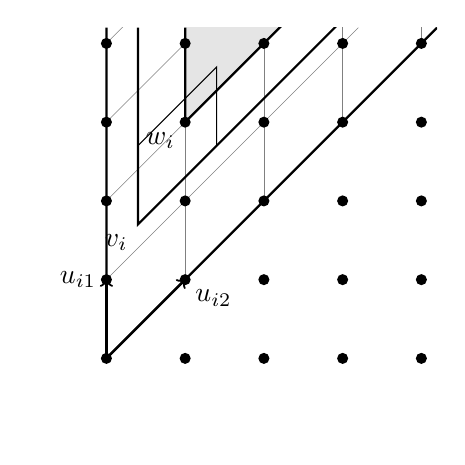
\begin{tikzpicture}
      \clip (-1,-1) rectangle (4.2,4.2);

      \foreach \y in {0,1,2,3,4}
        \draw[help lines] (0,\y) -- +(3.2,3.2);
      \foreach \x in {0,1,2,3,4}
        \draw[help lines] (\x,\x) -- +(0,3.2);

      \draw[thick,fill=black!10] (1,4.2) -- (1,3) node[below left] {$w_i$} -- +(4,4);

      \foreach \x in {0,1,...,4.01}
        \foreach \y in {0,1,...,4.01}
          \fill[black] (\x,\y) circle[radius=2pt];

      \draw[thick] (0,4.2) -- (0,0) -- (4.2,4.2);
      \draw[thick,->] (0,0) -- (0,1) node[left] {$u_{i1}$};
      \draw[thick,->] (0,0) -- (1,1) node[below right] {$u_{i2}$};

      \draw[thick] (0.4,4.2) -- (0.4,1.7) node[below left] {$v_i$} -- +(4,4);
      \draw (0.4,2.7) -- ++(1,1) -- ++(0,-1);
    \end{tikzpicture}
  \end{center}
  \caption{When a vertex $v_i$ is not integral, we obtain the generating function for $v_i + C_i$ by rounding to $w_i$.}
  \label{fig:unimodular-cone-apex-shift}
\end{figure}
In any case, there is a unique integer point $w_i$ in the translated fundamental parallelepiped $v_i + P(C_i)$,
see Figure~\ref{fig:unimodular-cone-apex-shift},
and
\[
  f(v_i + C_i;x) = f(w_i + C_i;x) = \frac{x^{w_i}}{\prod_{j=1}^d 1 - x^{u_{ij}}}
\]
because $v_i + C_i$ and $w_i + C_i$ contain the same integer points.

If we write
\[
  v_i = \sum_j \lambda_j u_{ij},
\]
then
\[
  w_i = \sum_j \lceil \lambda_j \rceil u_{ij}.
\]
The $\lambda$ are linear in $v_i$,
and $v_i$ is the solution of the system
\[
  A_{B_i} p = b_{B_i}
\]
associated to a basis of $v_i$.
That is, the $\lambda$ are linear in $b$.
Overall, we can find a matrix $T_i$ and a matrix $W_i$ such that
\[
  w_i = W_i \lceil T_i b \rceil,
\]
where the ceiling operation is component-wise.
We can now summarize:

\begin{theorem}
  \label{thm:rational-generating-function}
  Let $P = \{ p ~:~ Ax \leq b \} \subseteq \R^d$ be a rational polytope.
  Then
  \[
    f(P;x) = \sum_{i \in I} \varepsilon_i \frac{x^{w_i}}{\prod_{j=1}^d 1 - x^{u_{ij}}},
  \]
  where
  \begin{itemize}
    \item $\varepsilon_i = \pm1$ for all $i \in I$,
    \item the $u_{ij}$ span a unimodular cone for all $i \in I$, and
    \item $w_i = W_i \lceil T_i b \rceil$ for all $i \in I$,
  \end{itemize}
  where $W_i \in \Z^{d \times d}$ is unimodular and $T_i$ is a matrix
  such that $T_i b$ is integral if $P$ is an integral polytope.

  If $d$ is fixed, this formula for $f(P;x)$ can be computed in polynomial time.

  If the right hand side $b$ is changed without changing the combinatorial structure of $P$,
  then only the $w_i$ change as described by point~3.
\end{theorem}

In the last claim of Theorem~\ref{thm:rational-generating-function},
the combinatorial structure of $P$ refers means the set of bases of $A$ that give rise to vertices of $P$.
Changing the right hand side $b$ corresponds to a parallel translation of some of the inequalities that define $P$.
Such translations may cause new vertices to appear or old vertices to disappear.
However, as long as that does not happen, the underlying structure of $f(P;x)$ remains unchanged.

Counting the integer points in $P$ amounts to evaluating $f(P;1)$.
Unfortunately, the formula that we obtained is not defined at $x = 1$.
We solve this problem by replacing
\[
  x = g(t) := (e^{tc_1}, \ldots, e^{tc_d})
\]
for a suitable vector $c \in \Z^d$ and evaluating
\[
  |P \cap \Z^d| = \lim_{t \to 0} f(P; g(t)) = \lim_{t \to 0} \sum_{i \in I} \varepsilon_i \frac{e^{t c^Tv_i}}{\prod_j 1 - e^{t c^T u_{ij}}}
    = \lim_{t \to 0} \sum_{i \in I} \varepsilon_i \frac{e^{t \eta_i}}{\prod_j 1 - e^{t \mu_{ij}}}
\]
with $\eta_i$ and $\mu_{ij}$ appropriately defined.
Let us develop the power series of numerator and denominator:
\begin{align*}
  e^{t \eta_i} &= 1 + t\eta_i + t^2 \frac{\eta_i}{2} + \dots \\
  \prod_j 1 - e^{t \mu_{ij}} &= t^d (-1)^d \prod_j \mu_{ij} + \dots
\end{align*}
The power series of the numerator has a constant term,
while the power series of the denominator begins only at the $d$-th term,
and that only if all $\mu_{ij} \neq 0$.

\begin{lemma}
  We can choose $c \in \Z^d$ such that all $\mu_{ij} \neq 0$.
  This choice can be made in polynomial time.
\end{lemma}
\begin{proof}
  Consider $c(\lambda) := (\lambda, \lambda^2, \dots, \lambda^d)$.
  Given this choice of $c$,
  $\mu_{ij}$ is a non-zero polynomial in $\lambda$ of degree at most $d$.
  As a consequence, there are at most $d^2 |I|$ many values of $\lambda$ for which some $\mu_{ij} = 0$.
  After trying out polynomially many  integral values of $\lambda$,
  an appropriate $c \in \Z^d$ is found.
\end{proof}

Let us reformulate our limit as
\[
  |P \cap \Z^d| = \lim_{t \to 0} \frac{1}{t^d} \sum_{i \in I} \varepsilon_i \frac{t^d e^{t \eta_i}}{\prod_j 1 - e^{t \mu_{ij}}}
\]
so that now the power series of both the numerator and the denominator begin at the $d$-th term
in each summand.
As a consequence, we can write
\[
  |P \cap \Z^d| = \lim_{t \to 0} \frac{1}{t^d} \sum_{i \in I} \sum_{n=0}^\infty a_{in} t^n,
\]
for some $a_{in} \in \R$.
In fact, the $a_{in}$ can be computed using polynomial division applied to partial sums of the series.
For fixed $d$, this takes time that is polynomial in $n$,
where $n$ is the index of the largest coefficient that is to be computed,
and the encoding lengths of $\eta_i$ and the $\mu_{ij}$.
By analyzing this polynomial division, we also get:

\begin{fact}
  \label{fact:a_ik-polynomial}
  $a_{ik}$ is a polynomial in $\eta_i$ of degree at most $k$.
\end{fact}

Let $a_n := \sum_{i \in I} a_{in}$.
We already know that $t = 0$ is a removable singularity since the limit exists,
so we must have $a_0 = \dots = a_{d-1} = 0$. Furthermore,
\[
  |P \cap \Z^d| = a_d.
\]
We can now state the main algorithmic result of this chapter:

\begin{theorem}
  There is an algorithm that computes the number of integer points in a rational polytope
  in polynomial time in fixed dimension.
\end{theorem}

\begin{theorem}[Ehrhart polynomial]
  Let $P \subset \R^d$ be a full-dimensional integral polytope,
  that is, all vertices of $P$ are integer points.
  Then there is a polynomial $f$ of degree $d$
  such that
  \[
    |kP \cap \Z^d| = f(k)
  \]
  for all $k \in \N_{\geq 1}$.
\end{theorem}
\begin{proof}
  Notice that if $P = \{ p ~:~ Ap \leq b \}$ then $kP = \{ p ~:~ Ap \leq kb \}$.
  So $kP$ is obtained from $P$ by a linear change of the right hand side while keeping the combinatorial structure intact.
  As a consequence, the only change in the computation outlined above is in the $\eta_i$.
  Recall that
  \[
    \eta_i = c^T w_i = c^T W_i \lceil T_i b \rceil.
  \]
  However, since both $P$ and $kP$ for integral $k$ are integral polytopes,
  the ceiling operation is unnecessary.
  It follows that $\eta_i$ is a linear function in $k$,
  and so $f := a_d$ is a polynomial in $k$ of degree at most $d$ by Fact~\ref{fact:a_ik-polynomial}.

  An intuitive scaling argument shows that $f$ must be of degree exactly $d$:
  Since $P$ is a full-dimensional polytope, it contains a small rational cube $C$.
  Since $C$ is rational, there is an integer $M > 0$ such that $MC$ is integral with side length $N$.
  Therefore,
  \[
    f(kM) = |kM P \cap \Z^d| \geq |kMC \cap \Z^d| \geq (kN + 1)^d.
  \]
  Therefore, $f$ must be of degree at least $d$.
\end{proof}









\section*{Exercises}

\begin{enumerate}
  \item Show Lemma~\ref{lemma:cone-polars}.

  \item Show Lemma~\ref{lemma:simplicial-cone-polars}.

  \item Show the inclusion-exclusion formula (Lemma~\ref{lemma:inclusion-exclusion}).

  \item Show the remark after Corollary~\ref{corollary:cone-triangulation-series}:
    In the expression
    \[
      f(C;x) = \sum_{\emptyset \neq I \subseteq [n]} (-1)^{|I| - 1} f(\bigcap_{i \in I} C_i; x)
    \]
    for a triangulation of a pointed cone $C$,
    the trivial summands on the right hand side add up to $0$.

    \emph{Hint:} You can apply the Euler characteristic to the inclusion-exclusion formula applied to the vertex figure of the triangulation.

  \item Let $f \in \R\cP^d$ be such that the support of $f$ is restricted to a $k$-dimensional affine subspace $U \subset \R^d$.
    Let $\iota : \R^k \to U$ be an injective affine map.

    Show: $\mu(f) = \mu(f \circ \iota)$.

    \emph{Note:} The functions $\mu$ are defined on $\R\cP^d$ and $\R\cP^k$, respectively.

  \item Show: $[\relint P] \in \R\cP^d$ for all $P \in \cP^d$.

  \item In this problem, we explore an equivalent definition of the Euler characteristic
    and its implications.
    \begin{enumerate}[(a)]
      \item Let $\pi : \R^d \to \R$ be a projection, say on the first coordinate.
        For $f \in \R\cP_b^d$, let $\mu_t(f) := \mu_{d-1}(f|_{\pi^{-1}(t)})$, where $\mu_{d-1}$ is the $(d-1)$-dimensional Euler characteristic.

        Show: For all $f \in \R\cP_b^d$ one has $\mu(f) = \sum_{t \in \R} \mu_t(f) - \lim_{\varepsilon \to 0+} \mu_{t-\varepsilon}(f)$.

      \item Let $P \in \cP_b^d$ be a full-dimensional polytope.

        Show: $\mu([\operatorname{int} P]) = (-1)^d$.

      \item Let $f_0, \ldots, f_d \in \N_{\geq 0}$ be the so-called $f$-vector of $P$, that is,
        $f_j$ is the number of $j$-dimensional faces of $P$ (in particular, $f_0$ is the number of vertices and $f_d = 1$).

        Show the Euler formula $\sum_{j = 0}^d (-1)^j f_j = 1$.

      \item Extend the previous results to unbounded pointed polyhedra.

      \item Extend the previous results to general polyhedra.
    \end{enumerate}

  \item Show the Euler formula for planar graphs using the Euler characteristic.

  \item Show: Every simplicial cone $C \in \cP_v^d$ can be triangulated into unimodular cones.

  \item Show Lemma~\ref{lemma:simplicial-cone-signed-star}.

  \item Show: $\R \cP^d$ is an $\R$-algebra with operations $+$ and $\star$.
    Its neutral element is $1_\star = [\{0\}]$.

  \item Let $P \in \cP_b^d$ be a polytope. Show: $[P]$ is invertible with respect to $\star$.
    Its inverse is $(-1)^{\dim P} [\relint P]$.

  \item Let $\cD : \R \cP^d \to \R \cP^d$ be polarity (aka duality) and let $\cdot : \R \cP^d \to \R \cP^d$ be pointwise multiplication.
    \begin{enumerate}[(a)]
      \item
        Show: $\cD([K] \cdot [C]) = \cD([K]) \star \cD([C])$ and $\cD([K] \star [C]) = \cD([K]) \cdot \cD([C])$ for rational cones $K$ and $C$.

      \item
        Does the same relation hold for all $f, g \in \R \cP^d$?
    \end{enumerate}

  \item Let $c \in \R^d$.
    Show: There exists a unique linear map $LP_c: \R \cP_b^d \to \R$
    such that $LP_c([P]) = \max\{ c^Tx ~:~ x \in P \}$ for all $P \in \cP_b^d$.
\end{enumerate}
